\documentclass[aspectratio=169]{beamer}

% ---------- Pacotes ----------
\usepackage[utf8]{inputenc}
\usepackage[T1]{fontenc}
\usepackage[brazilian]{babel}
\usepackage{graphicx} % Required for inserting images
\usepackage{amsmath,amssymb,amsfonts}
\usepackage{booktabs}
\usepackage{tikz}
\usetikzlibrary{arrows.meta,positioning,calc,shapes.geometric}
\usepackage{pgfplots}
\pgfplotsset{compat=1.16}
\usepackage{algpseudocode}
\usepackage{listings}
\lstdefinestyle{py}{language=Python,basicstyle=\ttfamily\scriptsize,
  keywordstyle=\color{blue!60!black}\bfseries,commentstyle=\color{gray}\itshape,
  stringstyle=\color{red!55!black},showstringspaces=false,columns=fullflexible,
  keepspaces=true,frame=single,framerule=0.3pt,rulecolor=\color{gray!50},
  backgroundcolor=\color{gray!6},aboveskip=0pt,belowskip=0pt}
\lstdefinestyle{saida}{basicstyle=\ttfamily\scriptsize,columns=fullflexible,
  keepspaces=true,frame=single,framerule=0.3pt,rulecolor=\color{gray!50},
  aboveskip=0pt,belowskip=0pt}

\newtheorem{proposition}[theorem]{Proposição}

\usetheme{Madrid}

\title{Árvores de Decisão}
\subtitle{Da teoria do CART a bagging e boosting}
\author{Susaki, Salvo, Cunha}
\date{Outubro de 2026}

% ---------- Macros ----------
\DeclareMathOperator*{\argmin}{arg\,min}
\DeclareMathOperator*{\argmax}{arg\,max}
\newcommand{\ind}{\mathrm{I}}   % indicadora, como em Morettin \& Singer (eq. 10.1)
\newcommand{\E}{\mathbb{E}}
\newcommand{\Var}{\operatorname{Var}}
\newcommand{\R}{\mathbb{R}}
\newcommand{\Q}{Q}
\newcommand{\Err}{\mathcal E}
\newcommand{\Cand}{\mathcal C}            % medida de impureza
\newcommand{\TEC}{\mathrm{TEC}}
\newcommand{\cS}{\textcolor{blue!70!black}{S}} % saudável
\newcommand{\cD}{\textcolor{red!70!black}{D}}  % doente


% Numeração dos algoritmos (alterar aqui se a ordem mudar)
\newcommand{\aGrowZero}{1}
\newcommand{\aGrow}{2}
\newcommand{\aBest}{3}
\newcommand{\aPred}{4}
\newcommand{\aPrune}{5}
\newcommand{\aBag}{6}
\newcommand{\aRF}{7}
\newcommand{\aAda}{8}
\newcommand{\aGB}{9}

% Seções de código: apenas enumeradas (a preencher)
\newcounter{cb}
\newcommand{\ci}[2]{\stepcounter{cb}\item[\textbf{\thesection.\thecb}] #1\par{\scriptsize\color{gray}#2}}
\newcommand{\codeframe}[2]{%
  \setcounter{cb}{0}%
  \begin{frame}[t]{Código --- #1 \hfill {\scriptsize\color{gray}[a preencher]}}
  \footnotesize
  \begin{enumerate}
  #2
  \end{enumerate}
  \end{frame}}

% Gráfico de dispersão do exemplo (argumento: desenhos extras)
\newcommand{\scatterplot}[2][0.92\linewidth]{%
\begin{tikzpicture}
\begin{axis}[width=#1,height=6.2cm,xlabel={idade},ylabel={glicose},
  xmin=20,xmax=75,ymin=80,ymax=170,legend pos=north west,legend style={font=\scriptsize},
  tick label style={font=\scriptsize},label style={font=\small}]
\addplot[only marks,mark=*,blue!70!black,mark size=2.5pt] coordinates {(25,85)(41,92)(52,98)(63,125)(35,100)};
\addplot[only marks,mark=*,red!70!black,mark size=2.5pt] coordinates {(32,110)(45,150)(58,135)(67,160)(70,118)};
\legend{S,D}
#2
\end{axis}
\end{tikzpicture}}

\begin{document}

\maketitle

\begin{frame}{Roteiro}
\tableofcontents
\end{frame}

% =====================================================================
\section{Notação e definição}

\begin{frame}{Aprendizado supervisionado: notação}
\begin{itemize}
  \item Dados de treinamento $\mathcal D=\{(\mathbf x_i,y_i)\}_{i=1}^n$, com $\mathbf x_i=(x_{i1},\dots,x_{ip})^\top\in\R^p$.
  \item Cada \alert{linha} é uma observação (um ponto); cada \alert{coluna} preditora $X_j$ é um eixo do espaço $\R^p$.
  \item Resposta $Y$:
    \begin{itemize}
      \item \textbf{classificação}: $Y\in\{1,\dots,K\}$;
      \item \textbf{regressão}: $Y\in\R$.
    \end{itemize}
  \item Objetivo: construir $\hat f:\R^p\to Y$ com bom desempenho em dados \alert{novos}.
  \item Em geral: construção no conjunto de \textbf{treinamento}, avaliação em \textbf{validação/teste}.
\end{itemize}
\vfill
\end{frame}

\begin{frame}{exemplo}
\begin{columns}[c]
\column{0.38\textwidth}
\centering
\small
\begin{tabular}{rrrc}
\toprule
$i$ & idade & glicose & classe\\
\midrule
1 & 25 & 85  & \cS\\
2 & 32 & 110 & \cD\\
3 & 41 & 92  & \cS\\
4 & 45 & 150 & \cD\\
5 & 52 & 98  & \cS\\
6 & 58 & 135 & \cD\\
7 & 63 & 125 & \cS\\
8 & 67 & 160 & \cD\\
9 & 35 & 100 & \cS\\
10 & 70 & 118 & \cD\\
\bottomrule
\end{tabular}
\column{0.58\textwidth}
\centering
\scatterplot{}
\end{columns}
\vspace{2pt}
{\footnotesize $n=10$, $p=2$, $K=2$ (S = saudável, D = doente).}
\end{frame}

\begin{frame}{Definição: árvore binária de decisão}
\begin{definition}
Uma \alert{árvore de decisão binária} é uma árvore enraizada $T$ em que:
\begin{itemize}
  \item cada \alert{nó interno} $t$ está associado a uma \alert{divisão} $s_t=(j_t,\tau_t)$, com $j_t\in\{1,\dots,p\}$, e tem exatamente dois filhos:
  \[
  \text{esquerda: } \{\mathbf x: x_{j_t}<\tau_t\},\qquad \text{direita: } \{\mathbf x: x_{j_t}\ge\tau_t\};
  \]
  \item cada \alert{folha} (nó terminal) $m$ carrega um valor predito $c_m$.
\end{itemize}
\end{definition}
\begin{itemize}
  \item \textbf{Tamanho}: $|T|$ = número de folhas. \textbf{Profundidade}: maior número de arestas da raiz a uma folha.
  \item Notação: $M=|T|$ folhas; $\mathcal D_m$ = observações que chegam ao nó $m$; $n_m=|\mathcal D_m|$.
\end{itemize}
\end{frame}

\begin{frame}{Árvore $\Leftrightarrow$ partição do espaço}
\begin{columns}[c]
\column{0.50\textwidth}
\centering
\begin{tikzpicture}[
  int/.style={ellipse,draw,align=center,inner sep=2pt,font=\scriptsize},
  leaf/.style={rectangle,draw,align=center,inner sep=2.5pt,font=\scriptsize},
  level distance=1.15cm,
  level 1/.style={sibling distance=2.6cm},
  level 2/.style={sibling distance=2.2cm},
  level 3/.style={sibling distance=1.7cm},
  edge from parent/.style={draw,-{Latex[length=2mm]}}]
\node[int]{glicose $<105$?}
  child{node[leaf,fill=blue!10]{$R_1$: \cS\\$n=4$} edge from parent node[left,font=\tiny]{sim}}
  child{node[int]{idade $<60{,}5$?}
    child{node[leaf,fill=red!10]{$R_2$: \cD\\$n=3$} edge from parent node[left,font=\tiny]{sim}}
    child{node[int]{idade $<65$?}
      child{node[leaf,fill=blue!10]{$R_3$: \cS\\$n=1$} edge from parent node[left,font=\tiny]{sim}}
      child{node[leaf,fill=red!10]{$R_4$: \cD\\$n=2$} edge from parent node[right,font=\tiny]{não}}
      edge from parent node[right,font=\tiny]{não}}
    edge from parent node[right,font=\tiny]{não}};
\end{tikzpicture}
\column{0.48\textwidth}
\centering
\scatterplot[0.98\linewidth]{%
\addplot[black,dashed,thick] coordinates {(20,105)(75,105)};
\addplot[black,dashed,thick] coordinates {(60.5,105)(60.5,170)};
\addplot[black,dashed,thick] coordinates {(65,105)(65,170)};
\node[font=\scriptsize] at (axis cs:68,92) {$R_1$};
\node[font=\scriptsize] at (axis cs:30,138) {$R_2$};
\node[font=\tiny,fill=white,inner sep=0.5pt] at (axis cs:62.8,166) {$R_3$};
\node[font=\scriptsize] at (axis cs:72.5,140) {$R_4$};
}
\end{columns}
\vspace{2pt}
{\footnotesize Veremos (Seções~\ref{sec:ideia}--\ref{sec:cartdet}) como o CART constrói essa árvore a partir dos dados.}
% [MANIM] cada corte desenha uma região enquanto a árvore cresce ao lado
\end{frame}

\begin{frame}{O preditor $\hat f$ da árvore}
\begin{itemize}
  \item $\hat f$ é o \alert{preditor}: dado $\mathbf x=(x_1,\dots,x_p)$, devolve a previsão de $Y$, estimada a partir dos dados de treinamento.
  \item As folhas de $T$ definem $M$ regiões $R_1,\dots,R_M$ do espaço dos preditores: \alert{retângulos $p$-dimensionais} mutuamente exclusivos que o particionam.
  \item Para os pontos de $R_m$, o preditor de $Y$, que designamos $\hat Y_{R_m}$, é:
  \begin{itemize}
    \item a classe de $Y$ com \alert{maior frequência} entre os pontos de $R_m$ (resposta categorizada);
    \item a \alert{média} das respostas dos pontos de $R_m$ (resposta contínua).
  \end{itemize}
\end{itemize}
\begin{block}{Logo}
$\hat f(\mathbf x)=\hat Y_{R_m}$ \ se \ $\mathbf x\in R_m$: todos os pontos de uma região recebem a \alert{mesma} previsão.
\end{block}
\end{frame}

\begin{frame}{O preditor no exemplo}
Classificação, com as quatro regiões da árvore:

\vspace{8pt}
\centering
\begin{tabular}{@{}llc@{}}
\toprule
\textbf{Região} & \textbf{Condição} & $\hat f(\mathbf x)=\hat Y_{R_m}$\\
\midrule
$R_1$ & glicose $<105$ & \cS\\
$R_2$ & glicose $\ge105$ e idade $<60{,}5$ & \cD\\
$R_3$ & glicose $\ge105$ e $60{,}5\le$ idade $<65$ & \cS\\
$R_4$ & glicose $\ge105$ e idade $\ge65$ & \cD\\
\bottomrule
\end{tabular}

\vspace{10pt}
\raggedright
Cada região é um retângulo do plano (idade, glicose), e $\hat f$ é \alert{constante} dentro de cada um. Exemplo: um paciente com idade $63$ e glicose $125$ cai em $R_3$, logo $\hat f=\cS$.
\end{frame}

% =====================================================================
\section{Contexto histórico}

\begin{frame}{Por que árvores de decisão?}
\begin{columns}[T]
\column{0.48\textwidth}
\textbf{Vantagens}
\begin{itemize}
  \item Interpretáveis (regras ``se--então'').
  \item Captam não linearidades e interações sem especificá-las.
  \item Não exigem padronização das variáveis.
  \item Aceitam preditores numéricos e categóricos.
\end{itemize}
\column{0.48\textwidth}
\textbf{Limitações}
\begin{itemize}
  \item Alta variância: pequenas mudanças nos dados alteram a árvore.
  \item Fronteiras só paralelas aos eixos.
  \item Sobreajuste se a árvore cresce sem controle.
  \item Em geral, menos precisas que modelos mais flexíveis.
\end{itemize}
\end{columns}
\vfill
\begin{block}{Ideia central}
Particionar o espaço dos preditores em regiões simples e prever com uma constante em cada região.
\end{block}
\end{frame}

\begin{frame}{Panorama histórico}
\begin{itemize}
  \item \textbf{1960s--70s}: AID (Morgan \& Sonquist) --- divisões para regressão.
  \item \textbf{1984}: \alert{CART} (Breiman, Friedman, Olshen \& Stone) --- classificação e regressão, poda por custo-complexidade.
  \item \textbf{1986--93}: ID3 e C4.5 (Quinlan) --- ganho de informação, divisões multivia.
  \item \textbf{1996--2001}: bagging (Breiman), AdaBoost (Freund \& Schapire), florestas aleatórias (Breiman).
  \item \textbf{2001 em diante}: gradient boosting (Friedman) e implementações modernas (XGBoost, LightGBM, CatBoost).
\end{itemize}
% [MANIM] linha do tempo animada (opcional)
\end{frame}

% =====================================================================
\section{A ideia do algoritmo}\label{sec:ideia}

\begin{frame}{A ideia em quatro passos}
\textbf{Objetivo}: dividir o espaço dos preditores em regiões nas quais $Y$ é ``quase constante''.

\vspace{4pt}
\textbf{Estratégia}: em vez de procurar a partição inteira de uma só vez, \alert{dividir o espaço aos poucos}:
\begin{enumerate}
  \item Comece com o espaço inteiro (todas as observações).
  \item Faça \alert{uma pergunta} sobre \alert{uma única} variável: ``$X_j<\tau$?''. A resposta divide a região em duas.
  \item Escolha a pergunta que \alert{minimiza o erro} da divisão resultante.
  \item Repita os passos 2 e 3 \alert{dentro de cada} sub-região (recursão).
\end{enumerate}
\begin{block}{Por enquanto, o erro é uma caixa-preta}
Nesta seção não definimos como o erro é medido nem como a minimização é feita. O foco é a \alert{estrutura} do algoritmo e a pergunta: \alert{quando ele para?}
\end{block}
% [MANIM] o espaço sendo cortado, passo a passo, com a árvore crescendo ao lado
\end{frame}

\begin{frame}{Uma pergunta divide a região}
\begin{columns}[c]
\column{0.58\textwidth}
\footnotesize
Seja $R_m\subset\R^p$ a região atual (no início, $R_1=\R^p$) e
\[
\mathcal D_m=\{i:\ \mathbf x_i\in R_m\},\qquad n_m=|\mathcal D_m| .
\]
Uma \alert{pergunta} é um par $q=(j,\tau)$, com $j\in\{1,\dots,p\}$ e $\tau\in\R$. Ela divide a região e as observações:
\begin{align*}
R_L(q)&=R_m\cap\{\mathbf x: x_j<\tau\}, & \mathcal D_L(q)&=\{i\in\mathcal D_m: x_{ij}<\tau\},\\
R_R(q)&=R_m\cap\{\mathbf x: x_j\ge\tau\}, & \mathcal D_R(q)&=\{i\in\mathcal D_m: x_{ij}\ge\tau\}.
\end{align*}
$\{R_L,R_R\}$ particiona $R_m$ e $\{\mathcal D_L,\mathcal D_R\}$ particiona $\mathcal D_m$. O corte é perpendicular ao eixo $X_j$.
\column{0.40\textwidth}
\centering
\scatterplot[0.98\linewidth]{%
\addplot[black,dashed,thick] coordinates {(20,105)(75,105)};
\node[font=\scriptsize,fill=white,inner sep=1pt] at (axis cs:66,92) {$R_L$};
\node[font=\scriptsize,fill=white,inner sep=1pt] at (axis cs:66,145) {$R_R$};
\node[font=\scriptsize,anchor=south east] at (axis cs:74.5,106) {$q=(\text{glicose},105)$};
}
\end{columns}
\end{frame}

\begin{frame}{Perguntas candidatas}
\begin{definition}
Uma pergunta $q$ é \alert{não trivial} para $\mathcal D_m$ se $\mathcal D_L(q)\ne\varnothing$ e $\mathcal D_R(q)\ne\varnothing$. O conjunto $\Cand(\mathcal D_m)$ reúne as perguntas não triviais, identificando as que produzem a mesma bipartição de $\mathcal D_m$.
\end{definition}
\begin{proposition}
Para preditores numéricos, $|\Cand(\mathcal D_m)|\le p\,(n_m-1)$. Em particular, $\Cand(\mathcal D_m)$ é \alert{finito}.
\end{proposition}
\begin{proof}[Ideia]
Para cada $j$, sejam $a_1<\dots<a_r$ ($r\le n_m$) os valores distintos de $x_{ij}$ em $\mathcal D_m$. Limiares $\tau\le a_1$ ou $\tau>a_r$ são triviais, e todo $\tau\in(a_k,a_{k+1}]$ dá a mesma bipartição. Restam $\le r-1\le n_m-1$ por variável.
\end{proof}
{\footnotesize Variáveis categóricas com $q$ níveis: $x_j\in S$ contra $x_j\notin S$, com $2^{q-1}-1$ perguntas (detalhes na Seção~\ref{sec:cartdet}).}
\end{frame}

\begin{frame}{Erro de uma divisão (por ora, abstrato)}
Fixe uma função
\[
\Err(\mathcal D_m;\,j,\tau)\in[0,\infty),
\]
o \alert{erro} de dividir $\mathcal D_m$ pela pergunta $(j,\tau)$. Quanto menor, melhor. A \alert{pergunta ótima} do nó é
\[
q^*(\mathcal D_m)\in\argmin_{(j,\tau)\in\Cand(\mathcal D_m)}\ \Err(\mathcal D_m;\,j,\tau).
\]
\begin{itemize}
  \item O mínimo existe sempre que $\Cand(\mathcal D_m)\ne\varnothing$, pois o conjunto é finito.
  \item Pode haver empate; fixamos uma regra de desempate determinística.
  \item Valor de uma folha: $c(\mathcal D_m)$ = classe majoritária (classificação) ou média das respostas (regressão).
\end{itemize}
\begin{block}{O que usaremos de $\Err$ por enquanto}
(i) é calculável para cada pergunta; (ii) $\Cand(\mathcal D_m)$ é finito. Definição concreta: Seção~\ref{sec:impureza}; cálculo eficiente do $\argmin$: Seção~\ref{sec:cartdet}.
\end{block}
\end{frame}

\begin{frame}[t]{Algoritmo \aGrowZero: versão ingênua (sem parada)}
\small
\begin{algorithmic}[1]
\Function{CresceÁrvore}{$\mathcal D_m$}
  \State $(j^*,\tau^*)\gets\argmin_{(j,\tau)\in\Cand(\mathcal D_m)}\ \Err(\mathcal D_m;\,j,\tau)$ \Comment{pergunta ótima}
  \State $\mathcal D_L\gets\{i\in\mathcal D_m: x_{ij^*}<\tau^*\}$; \quad $\mathcal D_R\gets\mathcal D_m\setminus\mathcal D_L$
  \State \Return \textsc{Nó}$\bigl(j^*,\tau^*,\ $\Call{CresceÁrvore}{$\mathcal D_L$}$,\ $\Call{CresceÁrvore}{$\mathcal D_R$}$\bigr)$
\EndFunction
\Statex
\State $T\gets$ \Call{CresceÁrvore}{$\mathcal D$} \Comment{chamada na raiz, com todas as observações}
\end{algorithmic}
\vspace{6pt}
\begin{itemize}
  \item Cada chamada: \alert{pergunta} $\to$ \alert{divide} $\to$ \alert{delega} cada metade a uma chamada do mesmo tipo, com menos dados.
  \item Falta algo: em que momento o algoritmo deixa de perguntar?
\end{itemize}
\end{frame}

\begin{frame}{A recursão passo a passo (exemplo)}
\begin{columns}[T]
\column{0.5\textwidth}
\centering
\scatterplot[0.98\linewidth]{%
\only<2->{\addplot[black,dashed,thick] coordinates {(20,105)(75,105)};}
\only<3->{\addplot[black,dashed,thick] coordinates {(60.5,105)(60.5,170)};}
\only<4->{\addplot[black,dashed,thick] coordinates {(65,105)(65,170)};}
}
\column{0.48\textwidth}
\small
\begin{enumerate}
  \item<1-> \textbf{Chamada na raiz}: $\mathcal D$ com $n=10$, mistura de \cS{} e \cD.
  \item<2-> A caixa-preta devolve $q^*=(\text{glicose},105)$. $\mathcal D_L=\{1,3,5,9\}$ é pura $\Rightarrow$ folha \cS. Segue com $\mathcal D_R$ ($n=6$).
  \item<3-> $q^*=(\text{idade},60{,}5)$. $\mathcal D_L=\{2,4,6\}$ é pura $\Rightarrow$ folha \cD. Segue com $n=3$.
  \item<4-> $q^*=(\text{idade},65)$ separa $\{7\}$ de $\{8,10\}$, ambos puros $\Rightarrow$ duas folhas. Fim.
\end{enumerate}
\vspace{4pt}
{\scriptsize As perguntas foram obtidas com o erro de Gini (Seção~\ref{sec:impureza}); aqui basta tomá-las como dadas.}
\end{columns}
% [MANIM] a mesma sequência animada, com a árvore crescendo em paralelo
\end{frame}

\begin{frame}{E quando não há mais o que perguntar?}
\small
\begin{lemma}
$\Cand(\mathcal D_m)=\varnothing$ se, e somente se, para todo $j$ os valores $x_{ij}$, $i\in\mathcal D_m$, são todos iguais (em particular, se $n_m=1$).
\end{lemma}
\begin{proof}
($\Leftarrow$) Todo $\tau$ deixa um lado vazio. ($\Rightarrow$) Se algum $j$ tem valores $a<b$, então $\tau=(a+b)/2$ deixa os dois lados não vazios.
\end{proof}
No Algoritmo~\aGrowZero, num nó assim:
\begin{itemize}
  \item só perguntas não triviais: o $\argmin$ é sobre o conjunto \alert{vazio} e o algoritmo não produz árvore finita;
  \item admitindo perguntas triviais: $\mathcal D_L=\mathcal D_m$, e \textsc{CresceÁrvore}$(\mathcal D_m)$ chama a si mesma com o mesmo argumento: \alert{recursão infinita}.
\end{itemize}
\begin{alertblock}{Sem condição de parada, a recursão não termina}
Todo conjunto finito de dados leva a um nó em que não há mais pergunta possível.
\end{alertblock}
\end{frame}

\begin{frame}[t]{Algoritmo \aGrow: com condição de parada}
\small
Condição de parada mínima: \textsc{Parar}$(\mathcal D_m)\ :\Longleftrightarrow\ \Cand(\mathcal D_m)=\varnothing$ \ ou \ o nó é \alert{puro} (todos os $y_i$ iguais). $\Cand=\varnothing$ \alert{garante} o término; a pureza evita perguntas sem ganho.
\footnotesize
\begin{algorithmic}[1]
\Function{CresceÁrvore}{$\mathcal D_m$}
  \If{\textsc{Parar}$(\mathcal D_m)$} \State \Return \textsc{Folha}$\bigl(c(\mathcal D_m)\bigr)$ \EndIf
  \State $(j^*,\tau^*)\gets\argmin_{(j,\tau)\in\Cand(\mathcal D_m)}\ \Err(\mathcal D_m;\,j,\tau)$
  \State $\mathcal D_L\gets\{i\in\mathcal D_m: x_{ij^*}<\tau^*\}$; \quad $\mathcal D_R\gets\mathcal D_m\setminus\mathcal D_L$
  \State \Return \textsc{Nó}$\bigl(j^*,\tau^*,\ $\Call{CresceÁrvore}{$\mathcal D_L$}$,\ $\Call{CresceÁrvore}{$\mathcal D_R$}$\bigr)$
\EndFunction
\end{algorithmic}
\end{frame}

\begin{frame}{O algoritmo termina}
\begin{theorem}
Com a condição de parada mínima, \textsc{CresceÁrvore}$(\mathcal D)$ termina e devolve uma árvore com profundidade $\le n-1$, no máximo $n$ folhas e no máximo $2n-1$ nós.
\end{theorem}
\begin{proof}
Se a chamada em $\mathcal D_m$ não pára, então $\Cand(\mathcal D_m)\ne\varnothing$ e a pergunta escolhida é não trivial: $1\le n_L,n_R\le n_m-1$. Logo, ao descer de um nó a um filho, o tamanho $n_m$ (inteiro positivo) cai pelo menos 1. Partindo de $n$, qualquer caminho tem no máximo $n-1$ arestas, e a recursão termina. As folhas definem subconjuntos \alert{não vazios e disjuntos} de $\mathcal D$, então são no máximo $n$; como cada nó interno tem exatamente 2 filhos, o total de nós é $2\cdot\#\text{folhas}-1\le2n-1$.
\end{proof}
\begin{itemize}
  \item O limite é atingido quando cada folha tem uma única observação: a árvore memoriza os dados (sobreajuste, Seção~\ref{sec:overfit}).
  \item Parar \alert{antes} (mais critérios de parada, poda) só diminui a árvore e preserva o término.
\end{itemize}
\end{frame}

\begin{frame}{Por que uma pergunta de cada vez? (estratégia gulosa)}
O problema global seria escolher a partição em $M$ regiões que minimiza o erro total:
\[
\min_{R_1,\dots,R_M}\ \sum_{m=1}^M \frac{n_m}{n}\,\operatorname{erro}(R_m) .
\]
\begin{itemize}
  \item Cresce de forma combinatória com $n$, $p$ e $M$, e a árvore binária \alert{ótima} é um problema NP-completo
\end{itemize}
\begin{block}{O que o Algoritmo~\aGrow{} faz}
Divisão binária \alert{recursiva}, \alert{de cima para baixo} e \alert{gulosa} (\emph{greedy}): em cada nó escolhe-se a melhor pergunta \alert{local}, sem avaliar se uma pergunta pior agora permitiria perguntas melhores depois.
\end{block}
\end{frame}

% =====================================================================
\section{Medidas de impureza}\label{sec:impureza}

\begin{frame}{Abrindo a caixa-preta}
Na Seção~\ref{sec:ideia}, o erro $\Err(\mathcal D_m;j,\tau)$ ficou abstrato. Vamos defini-lo.

\vspace{6pt}
Dada uma \alert{medida de impureza} $\Q$ de um nó (pequena quando o nó é dominado por uma classe), o erro de uma pergunta $q=(j,\tau)$ é a impureza \alert{ponderada} dos dois filhos:
\[
\Err(\mathcal D_m;j,\tau)=\frac{n_L}{n_m}\,\Q(\mathcal D_L)+\frac{n_R}{n_m}\,\Q(\mathcal D_R),\qquad n_L=|\mathcal D_L(q)|,\ n_R=|\mathcal D_R(q)|.
\]
\begin{itemize}
  \item Minimizar $\Err$ equivale a maximizar a \alert{redução de impureza} $\Q(\mathcal D_m)-\Err(\mathcal D_m;j,\tau)$.
  \item Falta escolher $\Q$: erro de classificação, Gini ou entropia.
\end{itemize}
\end{frame}

\begin{frame}{Proporções no nó e regra de classificação}
Para o nó $m$ (região $R_m$) com $n_m$ observações e $K$ classes:
\[
\hat p_{mk}=\frac1{n_m}\sum_{\mathbf x_i\in R_m}\ind(y_i=k),\qquad k=1,\dots,K,
\qquad \sum_k\hat p_{mk}=1.
\]
\begin{itemize}
  \item Classe majoritária: $k(m)=\argmax_k \hat p_{mk}$.
  \item \textbf{Taxa de erros de classificação} no nó:
  \[
  \TEC_m=1-\max_k\hat p_{mk}.
  \]
\end{itemize}
\end{frame}

\begin{frame}{Índice de Gini e entropia}
Uma \alert{medida de impureza} $\Q(\hat{\mathbf p}_m)$ é pequena quando o nó é dominado por uma classe.
\begin{align*}
\text{Erro (TEC):}\quad & \Q_{\TEC}=1-\max_k\hat p_{mk}\\
\text{Gini:}\quad & G_m=\sum_{k=1}^K \hat p_{mk}(1-\hat p_{mk})=1-\sum_{k=1}^K\hat p_{mk}^2\\
\text{Entropia (cruzada):}\quad & D_m=-\sum_{k=1}^K\hat p_{mk}\log\hat p_{mk}\quad(0\log0:=0)
\end{align*}
\begin{itemize}
  \item Os três valem $0$ em um nó \alert{puro} ($\hat p_{mk}=1$ para algum $k$).
  \item Máximo no caso uniforme $\hat p_{mk}=1/K$: $\TEC=1-\tfrac1K$, $G=1-\tfrac1K$, $D=\log K$.
\end{itemize}
{\footnotesize Para $K=2$ e $\hat p=\hat p_{m1}$: $G=2\hat p(1-\hat p)$.}
\end{frame}

\begin{frame}{Comparação das medidas ($K=2$)}
\centering
\begin{tikzpicture}
\begin{axis}[width=0.62\textwidth,height=6.3cm,xlabel={$\hat p$ (proporção da classe 1)},
  ylabel={impureza},domain=0.001:0.999,samples=200,xmin=0,xmax=1,ymin=0,ymax=0.6,
  legend pos=south east,legend style={font=\scriptsize},tick label style={font=\scriptsize}]
\addplot[thick,black,dashed]{min(x,1-x)};
\addplot[thick,blue!70!black]{2*x*(1-x)};
\addplot[thick,red!70!black]{-(x*ln(x)+(1-x)*ln(1-x))/(2*ln(2))};
\legend{Erro (TEC),Gini,{Entropia $\div 2$ (bits)}}
\end{axis}
\end{tikzpicture}

{\footnotesize A entropia foi dividida por 2 para ficar na mesma escala. Gini e entropia são curvas suaves e estritamente côncavas; o erro é linear por partes.}
% [MANIM] ponto p deslizando e as três curvas sendo lidas
\end{frame}

\begin{frame}{Propriedades (por que Gini e entropia?)}
\begin{proposition}
$G(\mathbf p)=1-\sum_k p_k^2$ e $D(\mathbf p)=-\sum_k p_k\log p_k$ são \alert{estritamente côncavas} no simplex; $\Q_{\TEC}$ é côncava, mas não estritamente.
\end{proposition}

\begin{itemize}
  \item A concavidade garante que dividir nunca \alert{aumenta} a impureza ponderada (próximo slide).
  \item O erro é pouco sensível: várias divisões úteis podem ter o mesmo $\TEC$ ponderado.
  \item Por isso, para \alert{crescer} a árvore usa-se Gini/entropia; o $\TEC$ é mais usado na \alert{poda}.
\end{itemize}
\end{frame}

\begin{frame}{Redução de impureza de uma divisão}
Divisão $s=(j,\tau)$ do nó $m$ em filhos $L$ e $R$, com $\lambda=n_L/n_m$:
\[
\Err(\mathcal D_m;j,\tau)\equiv\Q_s=\frac{n_L}{n_m}\Q_L+\frac{n_R}{n_m}\Q_R,\qquad
\Delta(s,m)=\Q_m-\Q_s .
\]
\begin{proposition}
Se $\Q$ é côncava, então $\Delta(s,m)\ge 0$ para toda divisão $s$.
\end{proposition}
\begin{proof}
O vetor de proporções do pai é combinação convexa: $\hat{\mathbf p}_m=\lambda\hat{\mathbf p}_L+(1-\lambda)\hat{\mathbf p}_R$. Pela concavidade, $\Q(\hat{\mathbf p}_m)\ge\lambda\Q(\hat{\mathbf p}_L)+(1-\lambda)\Q(\hat{\mathbf p}_R)$.
\end{proof}
\begin{itemize}
  \item Com entropia, $\Delta$ é o \alert{ganho de informação} (ID3/C4.5).
  \item Estritamente côncava e $\hat{\mathbf p}_L\ne\hat{\mathbf p}_R$ $\Rightarrow$ $\Delta>0$ (o erro pode dar $\Delta=0$ numa divisão útil).
\end{itemize}
\end{frame}

\begin{frame}{Exemplo: raiz do exemplo}
Raiz: $n=10$, $5$ doentes. $\hat p_{\cD}=\tfrac12$, logo $G=0{,}5$, $D=1$ bit, $\TEC=0{,}5$.

\vspace{4pt}
\centering
\small
\begin{tabular}{lccc}
\toprule
\textbf{Corte candidato} & \textbf{esq.\ $n_L$ (D)} & \textbf{dir.\ $n_R$ (D)} & \textbf{$G$ ponderado}\\
\midrule
glicose $<105$ & 4 (0) & 6 (5) & \alert{0,167}\\
glicose $<99$  & 3 (0) & 7 (5) & 0,286\\
glicose $<130$ & 7 (2) & 3 (3) & 0,286\\
idade $<43$    & 4 (1) & 6 (4) & 0,417\\
idade $<65$    & 8 (3) & 2 (2) & 0,375\\
\bottomrule
\end{tabular}

\vspace{6pt}
\raggedright
Melhor corte: glicose $<105$. $G_L=0$, $G_R=2\cdot\tfrac56\cdot\tfrac16=\tfrac{5}{18}\approx0{,}278$,
\[
G_s=0{,}4\cdot0+0{,}6\cdot0{,}278\approx0{,}167,\qquad \Delta=0{,}5-0{,}167\approx0{,}333 .
\]
{\footnotesize Mesmo corte com outras medidas: $\TEC$ ponderado $=0{,}1$; entropia ponderada $\approx0{,}390$ bit (ganho $\approx0{,}610$ bit).}
\end{frame}



% =====================================================================
\section{CART em detalhe}\label{sec:cartdet}

\begin{frame}[t]{Algoritmo \aBest: a pergunta ótima (\textsc{MelhorCorte})}
\footnotesize
\begin{algorithmic}[1]
\Function{MelhorCorte}{$\mathcal D_m$}
  \State $(j^*,\tau^*,s^*)\gets(\varnothing,\varnothing,+\infty)$
  \For{$j=1,\dots,p$}
    \If{$X_j$ numérica ou ordinal}
      \State ordenar $\mathcal D_m$ por $x_{\cdot j}$; \ $\mathbf c_L\gets\mathbf 0$; \ $\mathbf c_R\gets$ contagens de classe de $\mathcal D_m$
      \For{$i=1,\dots,n_m-1$}
        \State mover a $i$-ésima observação de $R$ para $L$ \Comment{atualiza $\mathbf c_L,\mathbf c_R$}
        \If{$x_{(i)j}<x_{(i+1)j}$}
          \State $\tau\gets(x_{(i)j}+x_{(i+1)j})/2$; \ $s\gets\frac{n_L}{n_m}\Q(\mathbf c_L)+\frac{n_R}{n_m}\Q(\mathbf c_R)$
          \State \textbf{se} $s<s^*$ \textbf{então} $(j^*,\tau^*,s^*)\gets(j,\tau,s)$
        \EndIf
      \EndFor
    \Else \Comment{categórica}
      \State ordenar níveis por $\hat p_{c1}$; testar os $q-1$ cortes (Breiman)
    \EndIf
  \EndFor
  \State \Return $(j^*,\tau^*,s^*)$
\EndFunction
\end{algorithmic}
\end{frame}

\begin{frame}{Critérios de parada usuais}
O Algoritmo~\aGrow{} usa a condição \alert{mínima} ($\Cand=\varnothing$ ou nó puro). Na prática acrescentam-se outras, que interrompem o crescimento mais cedo:
\begin{enumerate}
  \item $n_m<n_{\min}^{\text{split}}$ (poucos elementos para dividir);
  \item algum filho teria menos de $n_{\min}^{\text{folha}}$ observações;
  \item $h\ge h_{\max}$ (profundidade máxima);
  \item o ganho $\Delta$ da melhor pergunta é menor que $\varepsilon$.
\end{enumerate}
\vspace{6pt}
\begin{itemize}
  \item São os \alert{hiperparâmetros de pré-poda}; Veremos eles mais para frente em bibliotecas como o scikit learn.
  \item Parar mais cedo não afeta o término (o teorema continua valendo).
  \item Sem eles, a árvore cresce até folhas puras e pode ter até $n$ folhas.
\end{itemize}
\end{frame}

\begin{frame}[t]{Algoritmo \aPred: predição}
\small
\begin{algorithmic}[1]
\Function{Prediz}{$T,\mathbf x$}
  \State $t\gets$ raiz de $T$
  \While{$t$ não é folha}
    \If{$x_{j_t}<\tau_t$} \State $t\gets$ filho esquerdo de $t$
    \Else \State $t\gets$ filho direito de $t$
    \EndIf
  \EndWhile
  \State \Return $c_t$ \Comment{$k(m)$ na classificação, $\bar y_m$ na regressão}
\EndFunction
\end{algorithmic}
\vspace{8pt}
\begin{itemize}
  \item Custo: $O(h)$ por observação, com $h$ a profundidade da árvore.
  \item Probabilidades estimadas: devolver $\hat{\mathbf p}_m$ da folha em vez de $k(m)$.
\end{itemize}
\end{frame}

\begin{frame}{Execução com o erro de Gini (números)}
\small
\begin{enumerate}
  \item \textbf{Raiz} ($n=10$, 5 D, $G=0{,}5$). \textsc{MelhorCorte}: glicose $<105$, $G_s=0{,}167$. Esquerda: 4 \cS, pura $\Rightarrow$ folha $R_1$.
  \item \textbf{Direita} ($n=6$: 5 \cD, 1 \cS; $G\approx0{,}278$). Dois cortes empatam com $G_s\approx0{,}222$: idade $<60{,}5$ e glicose $<130$. \alert{Desempate}: primeiro encontrado (menor $j$) $\Rightarrow$ idade $<60{,}5$.
    Esquerda: 3 \cD, pura $\Rightarrow$ folha $R_2$.
  \item \textbf{Direita} ($n=3$: obs.\ 7, 8, 10; 2 \cD, 1 \cS; $G\approx0{,}444$). Corte idade $<65$ separa $\{7\}$ de $\{8,10\}$, $G_s=0$. Folhas puras $R_3$ e $R_4$.
\end{enumerate}
\vspace{4pt}
\begin{block}{Resultado}
$3$ divisões, $4$ folhas, profundidade $3$, $\TEC=0$ no treino --- exatamente a árvore do Slide ``Árvore $\Leftrightarrow$ partição''.
\end{block}
% [MANIM] varredura do limiar em cada eixo com a impureza ponderada em cada candidato
\end{frame}

\begin{frame}{Complexidade}
Em um nó com $n_m$ observações e $p$ preditores numéricos:
\begin{itemize}
  \item ordenar cada $X_j$: $O(n_m\log n_m)$;
  \item varredura com contagens acumuladas: $O(n_m K)$, pois cada candidato custa $O(K)$ em vez de reclassificar o nó;
  \item custo do nó: $O\bigl(p\,n_m(\log n_m+K)\bigr)$.
\end{itemize}
\vspace{4pt}
Em cada nível da árvore, os nós particionam as $n$ observações ($\sum_m n_m\le n$):
\[
\text{custo por nível}=O\bigl(p\,n(\log n+K)\bigr),
\qquad
\text{custo total}\approx O\bigl(h\,p\,n(\log n+K)\bigr).
\]
\begin{itemize}
  \item Para árvores balanceadas, $h\approx\log_2 M$; no pior caso, $h\approx n$.
  \item Implementações reduzem o custo ordenando cada $X_j$ \alert{uma vez} e propagando a ordem aos filhos.
\end{itemize}
\end{frame}

\begin{frame}{Preditores categóricos}
Divisão do nó: $x_j\in S$ contra $x_j\notin S$, com $S\subset\{1,\dots,q\}$.
\begin{itemize}
  \item Número de divisões distintas: $2^{q-1}-1$ ($q=10\Rightarrow 511$; $q=30\Rightarrow>5\times10^8$).
\end{itemize}
\begin{theorem}[Breiman et al., 1984]
Em regressão (RSS) ou classificação binária (Gini/entropia), ordene os níveis por $\bar y_c$ (ou $\hat p_{c1}$). A divisão ótima entre as $2^{q-1}-1$ possíveis está entre as $q-1$ da forma $\{c_{(1)},\dots,c_{(l)}\}$ \textit{versus} o resto.
\end{theorem}
\begin{itemize}
  \item Reduz a busca de exponencial para $O(q\log q)$ por variável.
  \item Para $K>2$ classes não há garantia; usam-se heurísticas.
  \item \alert{Cuidado}: níveis em excesso (CEP, identificadores) favorecem o sobreajuste e viesam a escolha de variável.
\end{itemize}
\end{frame}

\begin{frame}{Empates, valores ausentes e variáveis categóricas em Python}
\begin{itemize}
  \item \textbf{Empates}: dois cortes com o mesmo $s$ produzem árvores diferentes com o mesmo erro de treino (ver exemplo). Implementações fixam uma regra (primeiro encontrado) ou sorteiam a ordem das variáveis.
  \item \textbf{Valores ausentes} (CART): \alert{divisões substitutas} --- outros preditores que imitam o corte principal e são usados quando $x_{j^*}$ falta.
  \item \textbf{Em R}: \texttt{rpart} e \texttt{ctree} (\texttt{partykit}) tratam fatores diretamente.
  \item \textbf{Em Python}: a \texttt{DecisionTreeClassifier} clássica pede variáveis numéricas; é preciso codificar (\emph{one-hot}: um nível contra os demais; \emph{ordinal} só se houver ordem real). Usaremos o scikit learn para os exemplos.
\end{itemize}
\end{frame}

\section{Tamanho, profundidade e sobreajuste}\label{sec:overfit}

\begin{frame}{A árvore completa memoriza o treino}
\begin{proposition}
Se não existem $i\ne i'$ com $\mathbf x_i=\mathbf x_{i'}$ e $y_i\ne y_{i'}$, a árvore crescida sem critério de parada (exceto pureza) tem $\TEC=0$ no treinamento e no máximo $n$ folhas.
\end{proposition}
\begin{proof}[Ideia]
Enquanto um nó contém duas observações com classes diferentes, existe uma coordenada em que seus valores diferem e portanto um corte que as separa. O processo termina em folhas puras; cada divisão aumenta o número de folhas em 1 e cada folha tem $\ge1$ observação.
\end{proof}
\begin{itemize}
  \item Erro de treino zero \alert{não} significa bom desempenho em dados novos.
  \item Cada folha com poucas observações estima $\hat{\mathbf p}_m$ com muito ruído (alta variância).
\end{itemize}
\end{frame}

\begin{frame}{Compromisso viés--variância}
Em regressão, para um ponto fixo $\mathbf x_0$, com $Y_0=f(\mathbf x_0)+\varepsilon$, $\Var(\varepsilon)=\sigma^2$:
\[
\E\bigl[(Y_0-\hat f(\mathbf x_0))^2\bigr]=\underbrace{\sigma^2}_{\text{ruído}}+\underbrace{\bigl(\E\hat f(\mathbf x_0)-f(\mathbf x_0)\bigr)^2}_{\text{viés}^2}+\underbrace{\Var\bigl(\hat f(\mathbf x_0)\bigr)}_{\text{variância}}.
\]
\begin{itemize}
  \item \textbf{Árvore rasa}: poucas regiões, viés alto, variância baixa (\emph{underfitting}).
  \item \textbf{Árvore profunda}: muitas regiões, viés baixo, variância alta (\emph{overfitting}).
  \item A profundidade/tamanho é o \alert{parâmetro de complexidade}; o ideal é intermediário.
\end{itemize}
{\footnotesize Morettin \& Singer (2021, \S10.2): árvores menores têm menor variância e maior interpretabilidade, ao custo de pequeno aumento do viés.}
\end{frame}

\begin{frame}{Erro de treino e de teste versus complexidade}
\centering
\begin{tikzpicture}
\begin{axis}[width=0.66\textwidth,height=6.3cm,xlabel={complexidade (profundidade / nº de folhas)},ylabel={erro},
  domain=0:1,samples=100,xmin=0,xmax=1,ymin=0,ymax=0.55,xtick=\empty,ytick=\empty,
  legend pos=north east,legend style={font=\scriptsize}]
\addplot[thick,blue!70!black]{0.45*exp(-5*x)+0.02};
\addplot[thick,red!70!black]{0.12+0.40*exp(-6*x)+0.45*x^3};
\addplot[dashed,gray] coordinates {(0.40,0)(0.40,0.55)};
\node[font=\scriptsize,gray] at (axis cs:0.40,0.03) [anchor=west] {ponto ideal};
\node[font=\scriptsize,anchor=south] at (axis cs:0.12,0.02) {\emph{underfit}};
\node[font=\scriptsize,anchor=south] at (axis cs:0.86,0.02) {\emph{overfit}};
\legend{treino,teste}
\end{axis}
\end{tikzpicture}

{\footnotesize Ilustração \alert{esquemática} (curvas desenhadas à mão, não são dados reais)}
% [MANIM] fronteira de decisão se ajustando ao ruído enquanto as curvas divergem
\end{frame}

\begin{frame}{Pré-poda: hiperparâmetros}
Limitam o crescimento \alert{durante} \textsc{CresceÁrvore}:

\vspace{6pt}
\centering
\small
\begin{tabular}{p{0.34\textwidth}p{0.26\textwidth}p{0.30\textwidth}}
\toprule
\textbf{Efeito} & \textbf{R (\texttt{rpart})} & \textbf{Python (scikit-learn)}\\
\midrule
Profundidade máxima & \texttt{maxdepth} & \texttt{max\_depth}\\
Mín.\ de obs.\ para dividir & \texttt{minsplit} & \texttt{min\_samples\_split}\\
Mín.\ de obs.\ por folha & \texttt{minbucket} & \texttt{min\_samples\_leaf}\\
Ganho mínimo por divisão & \texttt{cp} (relativo) & \texttt{min\_impurity\_decrease}\\
\bottomrule
\end{tabular}

\vspace{8pt}
\raggedright
\begin{itemize}
  \item Simples, mas míope: um corte pouco útil agora pode viabilizar um ótimo depois.
  \item Alternativa: crescer uma árvore grande e \alert{podar} (próximo slide).
\end{itemize}
\end{frame}

\begin{frame}{Pós-poda por custo-complexidade}
Para $\alpha\ge0$, penalizar o tamanho:
\[
R_\alpha(T)=R(T)+\alpha\,|T|,\qquad R(T)=\sum_{m\in\text{folhas}(T)}\frac{n_m}{n}\,\TEC_m .
\]
\begin{itemize}
  \item $\alpha=0$: árvore completa. $\alpha\to\infty$: apenas a raiz.
  \item Para cada $\alpha$ existe uma subárvore $T_\alpha\preceq T_{\max}$ que minimiza $R_\alpha$, e as $T_\alpha$ formam uma sequência \alert{aninhada}
  \[
  T_{\max}=T_0\succeq T_1\succeq\cdots\succeq\{\text{raiz}\},
  \]
  correspondente a $0=\alpha_0<\alpha_1<\cdots$ (Breiman et al., 1984).
  \item $\alpha$ é escolhido por validação cruzada.
\end{itemize}
\end{frame}

\begin{frame}[t]{Algoritmo \aPrune: poda pelo elo mais fraco}
\small
Para um nó interno $t$: $R(t)$ = erro se $t$ virasse folha; $T_t$ = subárvore enraizada em $t$.
\begin{algorithmic}[1]
\State $T_0\gets T_{\max}$; \ $k\gets0$
\While{$|T_k|>1$}
  \For{cada nó interno $t$ de $T_k$}
    \State $g_k(t)\gets\dfrac{R(t)-R(T_{k,t})}{|T_{k,t}|-1}$ \Comment{aumento de erro por folha eliminada}
  \EndFor
  \State $\alpha_{k+1}\gets\min_t g_k(t)$
  \State $T_{k+1}\gets T_k$ sem as subárvores abaixo dos nós com $g_k(t)=\alpha_{k+1}$ (viram folhas)
  \State $k\gets k+1$
\EndWhile
\State escolher $\hat k$ (ou $\alpha$) por validação cruzada; \Return $T_{\hat k}$
\end{algorithmic}
\end{frame}

\begin{frame}{Escolha do tamanho por validação cruzada}
\begin{enumerate}
  \item Crescer $T_{\max}$ nos dados de treinamento e obter a sequência $\alpha_0<\alpha_1<\cdots$.
  \item Para cada dobra $v=1,\dots,V$: crescer e podar nos dados sem a dobra; medir o erro na dobra para cada $\alpha$ (nos pontos médios geométricos entre $\alpha$'s consecutivos).
  \item Erro CV de cada $\alpha$ = média nas $V$ dobras; escolher o $\alpha$ de menor erro.
  \item \alert{Regra do 1-EP}: escolher a árvore \emph{menor} cujo erro CV está a até 1 erro-padrão do mínimo.
\end{enumerate}
\vspace{6pt}
\begin{itemize}
  \item No \texttt{rpart}, a tabela e o gráfico de CV são \texttt{printcp} e \texttt{plotcp}, e a árvore podada vem de \texttt{prune}.
  \item No scikit-learn, \texttt{cost\_complexity\_pruning\_path} fornece os $\alpha$ efetivos e \texttt{ccp\_alpha} fixa a poda.
\end{itemize}
\end{frame}

% PENDENTE (sobreajuste e poda): curvas de erro de treino e teste em função da profundidade (max_depth de 1 a 15) -- Python: validation_curve; R: loop com rpart
% PENDENTE (sobreajuste e poda): fronteiras de decisão em 2D para profundidades 1, 3 e ilimitada -- Python: matplotlib; R: ggplot2
% PENDENTE (sobreajuste e poda): pré-poda, grade de min_samples_leaf/minbucket e efeito no erro de teste -- Python: GridSearchCV; R: caret::train
% PENDENTE (sobreajuste e poda): seleção de alpha por validação cruzada com a regra do 1-EP -- Python: cross_val_score; R: plotcp
\begin{frame}[fragile]{Exemplo em Python: poda por custo-complexidade (Alg.~\aPrune)}
\lstinputlisting[style=py,basicstyle=\ttfamily\fontsize{7}{8.4}\selectfont]{../python/poda/01_poda_ccp.py}
\begin{minipage}{0.5\linewidth}
\lstinputlisting[style=saida,basicstyle=\ttfamily\fontsize{7}{8.4}\selectfont]{../python/poda/outputs/01_poda_ccp.txt}
\end{minipage}\hfill
\begin{minipage}{0.47\linewidth}\footnotesize
Poda: $9\to4$ folhas; o teste muda em \alert{uma} flor de $38$ ($0{,}921\to0{,}895$).
\end{minipage}
\end{frame}

% =====================================================================
\section{Avaliação do classificador}

\begin{frame}{Matriz de confusão e métricas}
Caso binário (positivo = \cD):

\vspace{4pt}
\centering
\small
\begin{tabular}{r|cc}
 & \textbf{predito \cD} & \textbf{predito \cS}\\ \hline
\textbf{real \cD} & VP & FN\\
\textbf{real \cS} & FP & VN\\
\end{tabular}

\vspace{6pt}
\raggedright
\[
\text{Acurácia}=\frac{VP+VN}{n},\quad
\text{Sensibilidade}=\frac{VP}{VP+FN},\quad
\text{Especificidade}=\frac{VN}{VN+FP},
\]
\[
\text{Precisão}=\frac{VP}{VP+FP},\qquad
F_1=\frac{2\cdot\text{Precisão}\cdot\text{Sensibilidade}}{\text{Precisão}+\text{Sensibilidade}} .
\]
\begin{itemize}
  \item A acurácia engana com classes desbalanceadas; escolher a métrica conforme o custo dos erros.
\end{itemize}
\end{frame}


\begin{frame}{Curva ROC e importância de variáveis}
\textbf{ROC}: para cada limiar $c$ sobre $\hat p_{m,\cD}$, traçar sensibilidade versus $1-$especificidade; \textbf{AUC} = área sob a curva = probabilidade de um positivo ter escore maior que um negativo.

\vspace{8pt}
\textbf{Importância de uma variável $X_j$} (redução de impureza):
\[
I(X_j)=\sum_{t:\ j_t=j}\frac{n_t}{n}\,\Delta(s_t,t) .
\]
\begin{itemize}
  \item Soma, sobre os nós em que $X_j$ define o corte, do ganho ponderado.
  \item Tende a favorecer variáveis com muitos cortes possíveis (numéricas contínuas, categóricas com muitos níveis).
  \item Alternativa: importância por \alert{permutação} (isso é papo para florestas aleatórias).
\end{itemize}
\end{frame}

% =====================================================================
\section{Árvores de regressão}\label{sec:regressao}

\begin{frame}{Da classificação à regressão: o que muda?}
\begin{itemize}
  \item A resposta agora é \alert{numérica}. A árvore continua sendo uma partição do espaço em retângulos $p$-dimensionais.
  \item Em cada folha, a previsão deixa de ser uma \alert{classe} (a moda) e passa a ser um \alert{número}: a \alert{média} das respostas das observações que caíram ali.
  \item O erro deixa de contar acertos e passa a medir a \alert{distância} entre $y_i$ e a previsão: a impureza do nó é a \alert{variância}.
  \item Tudo o mais é reaproveitado: perguntas $x_j\le\tau$, busca gulosa, condição de parada, poda.
\end{itemize}
\vspace{4pt}
\begin{block}{Exemplo corrente: \emph{diabetes} (scikit-learn)}
$442$ pacientes. Resposta: \alert{progressão da doença} um ano após a coleta (índice numérico). Preditores: idade, sexo, IMC, pressão e $6$ medidas de sangue. Começamos só com o \alert{IMC}, para poder \alert{desenhar} o ajuste.
\end{block}
\end{frame}

\begin{frame}[fragile]{API do scikit-learn: \texttt{DecisionTreeRegressor}}
\begin{lstlisting}[style=py]
DecisionTreeRegressor(*, criterion='squared_error', splitter='best',
    max_depth=None, min_samples_split=2, min_samples_leaf=1,
    max_features=None, random_state=None, max_leaf_nodes=None,
    min_impurity_decrease=0.0, ccp_alpha=0.0, ...)
\end{lstlisting}
\vspace{2pt}
\footnotesize
\begin{tabular}{@{}p{0.26\linewidth}p{0.68\linewidth}@{}}
\toprule
\texttt{criterion} & \texttt{'squared\_error'}: variância (nosso $\mathrm{RSS}$); também \texttt{'absolute\_error'} (mediana) e \texttt{'poisson'}\\
\texttt{max\_depth} & profundidade máxima $h_{\max}$ (\texttt{None}: sem limite)\\
\texttt{min\_samples\_leaf} & mínimo de observações por folha\\
\texttt{ccp\_alpha} & $\alpha$ da poda por custo-complexidade\\
\midrule
métodos & \texttt{fit}, \texttt{predict}, \texttt{score} (devolve $R^2$)\\
atributos & \texttt{tree\_}, \texttt{get\_n\_leaves()}, \texttt{feature\_importances\_}\\
\bottomrule
\end{tabular}

\vspace{2pt}
{\scriptsize Compare com \texttt{DecisionTreeClassifier}: muda o \texttt{criterion} (\texttt{'gini'}, \texttt{'entropy'}).}
\end{frame}

\begin{frame}[fragile]{Exemplo em Python: uma árvore de profundidade 2}
\lstinputlisting[style=py]{../python/regressao/01_arvore_bmi.py}
\vspace{4pt}
\begin{itemize}
  \item \texttt{export\_text} imprime as regras da árvore ajustada (próximo slide).
  \item O RMSE é a raiz do erro quadrático médio no teste, na unidade de $y$.
\end{itemize}
\end{frame}

\begin{frame}[fragile]{Lendo o resultado}
\begin{columns}[T]
\column{0.46\textwidth}
\lstinputlisting[style=saida,basicstyle=\ttfamily\fontsize{7}{8.4}\selectfont]{../python/regressao/outputs/01_arvore_bmi.txt}
\column{0.52\textwidth}
\small
\begin{itemize}
  \item Quatro folhas, quatro previsões: $106{,}9$, $138{,}2$, $190{,}0$ e $271{,}1$. Cada uma é a \alert{média} de $y$ no treino na sua região do IMC.
  \item Primeiro corte em $\text{IMC}\le0{,}01$; depois em $-0{,}02$ e $0{,}07$: o algoritmo escolheu \alert{onde} cortar para minimizar o RSS.
  \item RMSE no teste $=62{,}7$ contra desvio-padrão de $y$ de $74{,}7$: a árvore explica \alert{pouco}, esperado com uma só variável.
  \item Duas perguntas: \alert{por que} esses cortes (metodologia e algoritmo)? \alert{Quantas} folhas usar (sobreajuste)?
\end{itemize}
\end{columns}
\end{frame}

\begin{frame}{Metodologia $\times$ algoritmo}
\begin{columns}[T]
\column{0.485\textwidth}
\begin{block}{Metodologia: \emph{o que queremos}}
\small
Um \alert{modelo} e um \alert{critério}:
\begin{itemize}
  \item modelo: $\hat f(\mathbf x)=\sum_{m=1}^M \bar y_m\,\ind(\mathbf x\in R_m)$, com $R_1,\dots,R_M$ retângulos disjuntos;
  \item critério: escolher $R_1,\dots,R_M$ que minimizam
  \[\mathrm{RSS}=\sum_m\sum_{\mathbf x_i\in R_m}(y_i-\bar y_m)^2 .\]
\end{itemize}
É um \alert{problema de otimização}. Não diz como resolvê-lo.
\end{block}
\column{0.485\textwidth}
\begin{block}{Algoritmo: \emph{como obtemos}}
\small
Uma \alert{receita} que aproxima a solução:
\begin{itemize}
  \item testar \alert{todas} as partições é inviável (cresce explosivamente com $n$ e $p$);
  \item então: busca \alert{gulosa}, de cima para baixo, em \alert{um corte por vez}: Alg.~\aGrow{} e \aBest;
  \item pare por $h_{\max}$, $n_{\min}$ ou nó puro; depois pode (Alg.~\aPrune).
\end{itemize}
Entrega uma árvore \alert{boa}, não necessariamente a de menor RSS.
\end{block}
\end{columns}
\vspace{4pt}
\centering\small
Mesma \alert{metodologia} $\Rightarrow$ algoritmos diferentes são possíveis (CART, ID3, C4.5, \dots). Mesmo \alert{algoritmo} $\Rightarrow$ metodologias diferentes (classificação e regressão).
\end{frame}

\begin{frame}{Metodologia: modelo e critério}
Resposta contínua. Em cada região, a previsão é a média:
\[
\hat f(\mathbf x)=\sum_{m=1}^M \bar y_m\,\ind(\mathbf x\in R_m),\qquad \bar y_m=\frac1{n_m}\sum_{\mathbf x_i\in R_m}y_i .
\]
O critério é a soma dos quadrados dos resíduos:
\[
\mathrm{RSS}=\sum_{m=1}^M\sum_{\mathbf x_i\in R_m}(y_i-\bar y_m)^2 .
\]
\begin{itemize}
  \item Por que a \alert{média}? Fixadas as regiões, $\bar y_m$ minimiza $\sum_{\mathbf x_i\in R_m}(y_i-c)^2$ em $c$: a média é a melhor constante.
  \item A impureza do nó é a \alert{variância}: $\Q_m=\dfrac1{n_m}\sum_{\mathbf x_i\in R_m}(y_i-\bar y_m)^2$.
\end{itemize}
{\footnotesize Morettin \& Singer (2021, \S10.4 e Nota de Capítulo~4).}
\end{frame}

\begin{frame}{Algoritmo: o mesmo, com outra impureza}
\begin{itemize}
  \item \textsc{CresceÁrvore} e \textsc{MelhorCorte} (Alg.~\aGrow{} e \aBest) valem sem mudanças, trocando $\Q$ por variância e $k(m)$ por $\bar y_m$.
  \item O melhor corte do nó minimiza $\mathrm{RSS}_L+\mathrm{RSS}_R$, equivalente a $\frac{n_L}{n_m}\Q_L+\frac{n_R}{n_m}\Q_R$.
  \item Varredura eficiente: manter $S_1=\sum y_i$ e $S_2=\sum y_i^2$ de cada lado; então
  \[
  \mathrm{RSS}_{\text{nó}}=S_2-\frac{S_1^2}{n_{\text{nó}}},
  \]
  e cada candidato custa $O(1)$.
  \item Poda por custo-complexidade: $R_\alpha(T)=\mathrm{RSS}(T)+\alpha|T|$, com o mesmo Algoritmo~\aPrune.
  \item Categóricas: níveis ordenados por $\bar y_c$ (teorema de Breiman, exato em regressão).
\end{itemize}
% [MANIM] corte candidato deslizando sobre o IMC e o RSS mudando
\end{frame}

\begin{frame}{A função em degraus, por profundidade}
\centering
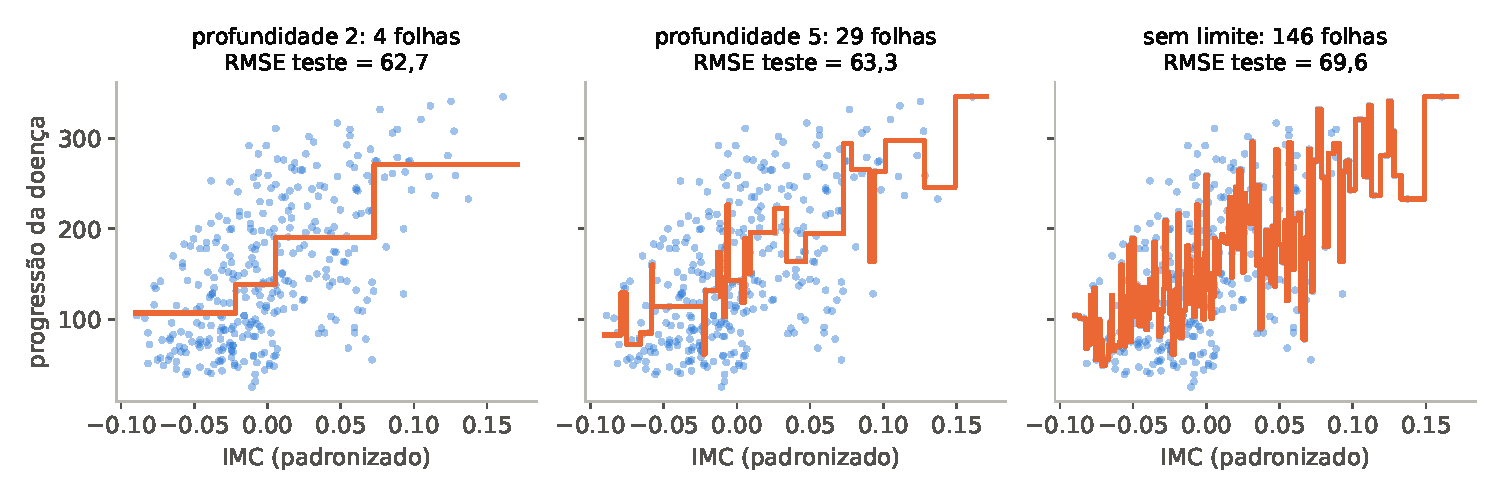
\includegraphics[width=\linewidth]{../python/regressao/figures/degraus.pdf}
\vspace{2pt}
\begin{itemize}
  \item Profundidade $2$: poucos degraus, curva grosseira (viés). Sem limite: $146$ folhas para $331$ pacientes de treino, \alert{decorando o ruído} (variância).
  \item O menor RMSE de teste está no meio. Próximo slide: em média de $30$ divisões.
\end{itemize}
% [MANIM] função em degraus aproximando os dados conforme a árvore cresce
\end{frame}

\begin{frame}[fragile]{Profundidade e sobreajuste em números}
\lstinputlisting[style=py,firstline=12,lastline=21]{../python/regressao/02_profundidade.py}
\vspace{3pt}
\lstinputlisting[style=saida]{../python/regressao/outputs/02_profundidade.txt}
\vspace{3pt}
{\small O RMSE de \alert{treino} só cai com a profundidade ($65{,}2\to47{,}0$); o de \alert{teste} cai até a profundidade $2$ ($64{,}3$) e sobe depois, chegando a $75{,}3$, perto do desvio-padrão de $y$.}
\end{frame}

\begin{frame}[fragile]{Escolhendo a complexidade por validação cruzada}
\lstinputlisting[style=py,firstline=9,lastline=16]{../python/regressao/03_validacao_cruzada.py}
\vspace{3pt}
\lstinputlisting[style=saida]{../python/regressao/outputs/03_validacao_cruzada.txt}
\vspace{3pt}
\begin{itemize}
  \item A validação cruzada ($5$ partes, só no treino) escolhe $h_{\max}=2$ e folhas com pelo menos $20$ pacientes.
  \item O RMSE no teste ($62{,}7$) fica próximo do estimado ($64{,}5$): a estimativa é honesta.
\end{itemize}
\end{frame}

\begin{frame}{Limitações das árvores de regressão}
\begin{block}{A função predita é descontínua e em degraus}
Não \alert{extrapola}: fora do intervalo do treino, devolve a média da folha de borda. Aproxima mal relações suaves ou lineares.
\end{block}
\begin{itemize}
  \item Uma única árvore é \alert{instável} (alta variância): $\Rightarrow$ bagging, florestas e boosting nas seções seguintes.
  \item No caso prático (Seção~\ref{sec:caso}), uma árvore completa tem RMSE \alert{pior} que uma reta com as $10$ variáveis.
\end{itemize}
\end{frame}


% =====================================================================
\section{Ensembles e bagging}\label{sec:bagging}

\begin{frame}{A sabedoria das multidões}
\begin{itemize}
  \item Faça uma pergunta difícil a milhares de pessoas e agregue as respostas. Em geral, a resposta agregada é \alert{melhor} que a de um único especialista: é a \emph{sabedoria das multidões}.
  \item Mesma ideia em aprendizado de máquina: agregue as previsões de um \alert{grupo de preditores}. O resultado costuma ser melhor que o do melhor preditor individual.
  \item Um grupo de preditores é um \alert{ensemble}, e o algoritmo que o constrói é um \alert{método de ensemble}.
  \item Por que interessa a árvores? Uma árvore é \alert{instável} (alta variância); combinar muitas pode compensar isso.
\end{itemize}
\vspace{4pt}
\centering
\begin{tikzpicture}[
  caixa/.style={draw,rounded corners=2pt,minimum height=0.6cm,inner sep=3pt,font=\small},
  seta/.style={-{Latex[length=1.8mm]}}]
\node[caixa] (x) at (0,0) {$\mathbf x$};
\node[caixa] (h1) at (3,0.9) {$h_1(\mathbf x)$};
\node[caixa] (h2) at (3,0) {$h_2(\mathbf x)$};
\node at (3,-0.55) {$\vdots$};
\node[caixa] (hB) at (3,-1.2) {$h_B(\mathbf x)$};
\node[caixa,fill=blue!8] (ag) at (6.4,0) {agregação};
\node[caixa] (y) at (9,0) {$\hat y(\mathbf x)$};
\foreach \h in {h1,h2,hB}{\draw[seta] (x) -- (\h); \draw[seta] (\h) -- (ag);}
\draw[seta] (ag) -- (y);
\end{tikzpicture}

% [MANIM] a multidão de preditores votando
\end{frame}

\begin{frame}{Votação por maioria (\emph{hard voting})}
Sejam $h_1,\dots,h_B:\R^p\to\{1,\dots,K\}$ classificadores treinados. O \alert{classificador por votação} devolve a classe mais votada (a moda):
\[
\hat y(\mathbf x)=\argmax_{k}\ \sum_{b=1}^{B}\ind\bigl(h_b(\mathbf x)=k\bigr).
\]
\begin{itemize}
  \item Exemplo com $B=3$: votos $1,0,1\ \Rightarrow\ \hat y=1$.
  \item Surpresa: o ensemble pode superar \alert{até o melhor} membro, mesmo que cada membro seja individualmente fraco.
  \item Quando isso acontece? Veja o próximo slide.
\end{itemize}
\end{frame}

\begin{frame}{Por que funciona: lei dos grandes números}
\begin{columns}[T]
\column{0.47\textwidth}
\small
Suponha $B$ classificadores \alert{independentes}, cada um correto com probabilidade $p>\tfrac12$. O número de acertos é $X\sim\mathrm{Binomial}(B,p)$ e a maioria acerta se $X>B/2$:
\[
P(\text{maioria correta})=\sum_{k>B/2}\binom Bk p^k(1-p)^{B-k}.
\]
\begin{itemize}
  \item Pela lei dos grandes números, $X/B\to p>\tfrac12$, e portanto a probabilidade $\to1$ quando $B\to\infty$.
  \item Cota de Hoeffding: $\ \ge 1-e^{-2B(p-1/2)^2}$.
\end{itemize}
\column{0.52\textwidth}
\centering
\begin{tikzpicture}
\begin{axis}[width=\linewidth,height=5.6cm,xmode=log,
  xlabel={número de classificadores $B$},ylabel={$P(\text{maioria correta})$},
  ymin=0.45,ymax=1.03,ymajorgrids,grid style={gray!25},
  tick label style={font=\scriptsize},label style={font=\small},
  legend style={font=\scriptsize,at={(0.97,0.05)},anchor=south east,draw=none,fill=none}]
\addplot[thick,color={rgb,255:red,127;green,179;blue,232}] table[x=B,y=p51]{../python/ensembles/figures/maioria.dat};
\addplot[thick,color={rgb,255:red,42;green,120;blue,214}] table[x=B,y=p55]{../python/ensembles/figures/maioria.dat};
\addplot[thick,color={rgb,255:red,20;green,74;blue,143}] table[x=B,y=p60]{../python/ensembles/figures/maioria.dat};
\legend{$p=0{,}51$,$p=0{,}55$,$p=0{,}60$}
\end{axis}
\end{tikzpicture}
\end{columns}
\end{frame}

\begin{frame}[fragile]{Números: votos independentes}
\lstinputlisting[style=py,basicstyle=\ttfamily\footnotesize]{../python/ensembles/01_maioria.py}
\vspace{4pt}
{\footnotesize\textbf{Saída}}
\lstinputlisting[style=saida,basicstyle=\ttfamily\footnotesize]{../python/ensembles/outputs/01_maioria.txt}
\vspace{2pt}
\begin{itemize}
  \item Mesmo com $p=0{,}51$ (quase uma moeda), $B=10\,000$ votos dão $\approx97{,}7\%$ de chance de a maioria acertar.
\end{itemize}
\end{frame}

\begin{frame}{Atenção: a premissa é a independência}
\begin{itemize}
  \item Classificadores treinados nos \alert{mesmos dados}, com o mesmo algoritmo, tendem a cometer os \alert{mesmos erros}. Se erram juntos, a maioria erra junto.
  \item Exemplo: $B=3$ classificadores com acurácia $p=0{,}70$.
  \begin{itemize}
    \item independentes: $P(\text{maioria correta})=3p^2-2p^3=0{,}784$;
    \item idênticos: $0{,}700$ (a votação não ajuda).
  \end{itemize}
  \item Para ganhar com o ensemble é preciso \alert{diversidade}. Duas formas:
  \begin{enumerate}
    \item \alert{algoritmos diferentes} nos mesmos dados (votação);
    \item o \alert{mesmo algoritmo} em \alert{amostras diferentes} dos dados (bagging).
  \end{enumerate}
\end{itemize}
\end{frame}

\begin{frame}{Votação suave (\emph{soft voting})}
Se cada classificador estima probabilidades $\hat p_b(k\mid\mathbf x)$, podemos \alert{tirar a média} delas:
\[
\hat y(\mathbf x)=\argmax_{k}\ \frac1B\sum_{b=1}^{B}\hat p_b(k\mid\mathbf x).
\]
\begin{block}{Mini-exemplo ($B=3$, probabilidade da classe 1)}
$0{,}90,\ 0{,}45,\ 0{,}45$.\quad \textbf{Hard}: votos $1,0,0\Rightarrow$ classe $0$. \quad \textbf{Soft}: média $=0{,}60\Rightarrow$ classe $1$.
\end{block}
\begin{itemize}
  \item Dá mais peso a votos \alert{confiantes}. Exige que os membros tenham \texttt{predict\_proba}.
  \item A documentação do scikit-learn a recomenda para classificadores \alert{bem calibrados}.
  \item Árvores completas dão probabilidades $0$ ou $1$: pouca informação para a média.
\end{itemize}
\end{frame}

\begin{frame}[fragile]{API do scikit-learn: \texttt{VotingClassifier}}
\begin{lstlisting}[style=py]
from sklearn.ensemble import VotingClassifier

VotingClassifier(estimators, *, voting='hard', weights=None,
                 n_jobs=None, flatten_transform=True, verbose=False)
\end{lstlisting}
\vspace{2pt}
\footnotesize
\begin{tabular}{@{}p{0.2\linewidth}p{0.74\linewidth}@{}}
\toprule
\texttt{estimators} & lista de pares \texttt{(nome, classificador)}\\
\texttt{voting} & \texttt{'hard'}: maioria dos rótulos; \texttt{'soft'}: argmax da soma das probabilidades\\
\texttt{weights} & pesos opcionais dos membros (padrão: uniformes)\\
\texttt{n\_jobs} & paralelismo no \texttt{fit}\\
\midrule
métodos & \texttt{fit}, \texttt{predict}, \texttt{score}; \texttt{predict\_proba} apenas com \texttt{voting='soft'}\\
atributos & \texttt{estimators\_} (membros ajustados), \texttt{named\_estimators\_}, \texttt{classes\_}\\
\bottomrule
\end{tabular}

\vspace{2pt}
{\scriptsize Assinatura da versão 1.9 do scikit-learn; confira a documentação da sua versão.}
\end{frame}

\begin{frame}[fragile]{Exemplo em Python: votação}
\lstinputlisting[style=py]{../python/ensembles/02_votacao.py}
\vspace{2pt}
{\scriptsize Iris: 150 flores, 4 medidas, 3 espécies; 112 para treino e 38 para teste.}
\end{frame}

\begin{frame}[fragile]{Resultado da votação (uma divisão)}
\lstinputlisting[style=saida]{../python/ensembles/outputs/02_votacao.txt}
\vspace{4pt}
\begin{itemize}
  \item \textbf{Hard} ($0{,}947$) empata com a regressão logística e fica abaixo do KNN ($0{,}974$); \textbf{soft} ($0{,}921$) fica abaixo de ambos.
  \item Cuidado: o teste tem $38$ flores, então \alert{uma} observação vale $\approx2{,}6$ pontos percentuais. Uma única divisão não decide nada.
  \item Próximo slide: repetir com $100$ divisões diferentes.
\end{itemize}
\end{frame}

\begin{frame}[fragile]{Repetindo 100 divisões treino/teste}
\lstinputlisting[style=py,firstline=16,lastline=24]{../python/ensembles/02b_votacao_repetido.py}
\vspace{3pt}
\lstinputlisting[style=saida]{../python/ensembles/outputs/02b_votacao_repetido.txt}
\vspace{3pt}
{\small A votação \alert{não} supera o melhor membro (KNN, $0{,}966$) e fica a $\approx0{,}003$ da média dos três ($0{,}959$), bem dentro do desvio-padrão ($\approx0{,}03$). No Iris os membros já acertam $\approx95$--$97\%$; nas $100$ divisões, \alert{todos} os erros caem em \emph{versicolor} $\times$ \emph{virginica} e $41\%$ das flores erradas por algum membro são erradas pelos \alert{três}: pouca diversidade, pouco a ganhar.}
\end{frame}

\begin{frame}{De votação a bagging: um algoritmo, dados diferentes}
\begin{itemize}
  \item \alert{Bagging} (\emph{bootstrap aggregating}, Breiman, 1996): treinar o \alert{mesmo} algoritmo em $B$ amostras aleatórias \alert{com reposição} do treino.
  \item \alert{Pasting}: o mesmo, mas amostras \alert{sem reposição}.
  \item Agregação: \alert{moda} (classificação) ou \alert{média} (regressão).
  \item Cada árvore vê dados diferentes, logo é diferente: a diversidade vem dos \alert{dados}.
\end{itemize}
\vspace{2pt}
\centering
\begin{tikzpicture}[
  caixa/.style={draw,rounded corners=2pt,minimum height=0.6cm,inner sep=3pt,font=\small},
  seta/.style={-{Latex[length=1.8mm]}}]
\node[caixa] (D) at (0,0) {$\mathcal D$};
\node[caixa] (d1) at (2.4,0.9) {$\mathcal D^{*1}$};
\node[caixa] (d2) at (2.4,0) {$\mathcal D^{*2}$};
\node at (2.4,-0.55) {$\vdots$};
\node[caixa] (dB) at (2.4,-1.2) {$\mathcal D^{*B}$};
\node[caixa] (t1) at (4.8,0.9) {$T_1$};
\node[caixa] (t2) at (4.8,0) {$T_2$};
\node at (4.8,-0.55) {$\vdots$};
\node[caixa] (tB) at (4.8,-1.2) {$T_B$};
\node[caixa,fill=blue!8] (ag) at (7.4,0) {agregação};
\foreach \d/\t in {d1/t1,d2/t2,dB/tB}{\draw[seta] (D) -- (\d); \draw[seta] (\d) -- (\t); \draw[seta] (\t) -- (ag);}
\end{tikzpicture}
% [MANIM] amostras bootstrap gerando árvores diferentes
\end{frame}

\begin{frame}{Árvores são instáveis: bootstrap}
\begin{itemize}
  \item Dividir aleatoriamente os dados em dois e ajustar duas árvores pode dar resultados bem diferentes: \alert{alta variância}.
  \item \textbf{Bootstrap}: amostra $\mathcal D^{*}$ de tamanho $n$, \alert{com reposição}, de $\mathcal D$.
  \item Probabilidade de uma observação \alert{não} entrar em $\mathcal D^*$:
  \[
  \Bigl(1-\frac1n\Bigr)^n\xrightarrow[n\to\infty]{}e^{-1}\approx0{,}368 .
  \]
  Logo, cerca de $63{,}2\%$ das observações distintas aparecem em cada amostra.
\end{itemize}
{\footnotesize Morettin \& Singer (2021, \S10.3.1 e Nota de Capítulo~3).}
\end{frame}

\begin{frame}[fragile]{Bootstrap em Python}
\lstinputlisting[style=py,basicstyle=\ttfamily\footnotesize]{../python/ensembles/03_bootstrap.py}
\vspace{4pt}
{\footnotesize\textbf{Saída}}
\lstinputlisting[style=saida,basicstyle=\ttfamily\footnotesize]{../python/ensembles/outputs/03_bootstrap.txt}
\vspace{2pt}
\begin{itemize}
  \item A fração de observações distintas converge para $1-1/e\approx0{,}632$.
\end{itemize}
\end{frame}

\begin{frame}[t]{Algoritmo \aBag: bagging}
\small
\begin{algorithmic}[1]
\For{$b=1,\dots,B$}
  \State $\mathcal D^{*b}\gets$ amostra bootstrap de $\mathcal D$ \Comment{$n$ sorteios com reposição}
  \State $T_b\gets$ \Call{CresceÁrvore}{$\mathcal D^{*b}$} \Comment{profunda, em geral sem poda}
\EndFor
\State \textbf{Classificação}: $\hat f_{\text{bag}}(\mathbf x)=\text{moda}\{T_1(\mathbf x),\dots,T_B(\mathbf x)\}$
\State \textbf{Regressão}: $\hat f_{\text{bag}}(\mathbf x)=\dfrac1B\sum_{b=1}^B T_b(\mathbf x)$
\Statex
\State \textbf{Erro OOB}: para cada $i$, prever $\mathbf x_i$ só com as árvores $T_b$ tais que $i\notin\mathcal D^{*b}$; comparar com $y_i$
\end{algorithmic}
\vspace{6pt}
\begin{itemize}
  \item As $B$ árvores são geradas \alert{independentemente} (paralelizável).
  \item O erro OOB é uma estimativa de erro de teste sem separar um conjunto de validação.
\end{itemize}
\end{frame}

\begin{frame}[fragile]{API do scikit-learn: \texttt{BaggingClassifier}}
\begin{lstlisting}[style=py]
BaggingClassifier(estimator=None, n_estimators=10, *, max_samples=None,
                  max_features=1.0, bootstrap=True, bootstrap_features=False,
                  oob_score=False, warm_start=False, n_jobs=None,
                  random_state=None, verbose=0)
\end{lstlisting}
\vspace{2pt}
\footnotesize
\begin{tabular}{@{}p{0.24\linewidth}p{0.70\linewidth}@{}}
\toprule
\texttt{estimator} & algoritmo base (aqui, \texttt{DecisionTreeClassifier()})\\
\texttt{n\_estimators} & número $B$ de preditores\\
\texttt{max\_samples} & tamanho de cada amostra; \texttt{None} $=n$ (como no Algoritmo~\aBag)\\
\texttt{bootstrap} & \texttt{True}: \alert{bagging} (com reposição); \texttt{False}: \alert{pasting}\\
\texttt{oob\_score} & calcula a acurácia \emph{out-of-bag} (só com \texttt{bootstrap=True})\\
\texttt{n\_jobs} & paralelismo ($-1$: todos os núcleos)\\
\bottomrule
\end{tabular}

\vspace{4pt}
\begin{itemize}
  \item \texttt{predict}: classe de maior probabilidade \alert{média}; sem \texttt{predict\_proba} no estimador base, usa votação.
\end{itemize}
{\scriptsize Versão 1.9; em versões antigas o argumento chamava-se \texttt{base\_estimator} e \texttt{max\_samples} valia $1{,}0$.}
\end{frame}

\begin{frame}[fragile]{Exemplo em Python: árvore única $\times$ bagging}
\lstinputlisting[style=py]{../python/ensembles/04_bagging.py}
\vspace{4pt}
\lstinputlisting[style=saida]{../python/ensembles/outputs/04_bagging.txt}
{\footnotesize No teste, $0{,}895\to0{,}947$: \alert{2 flores} de diferença em $38$. Confira com repetições no próximo slide.}
\end{frame}

\begin{frame}[fragile]{Repetindo: quando o bagging ajuda?}
\lstinputlisting[style=py,firstline=10,lastline=21]{../python/ensembles/04b_bagging_repetido.py}
\vspace{3pt}
\lstinputlisting[style=saida]{../python/ensembles/outputs/04b_bagging_repetido.txt}
\vspace{3pt}
{\small Com as $4$ variáveis a árvore já é boa e o ganho é pequeno ($+0{,}007$, menor que o desvio-padrão). Só com as \alert{sépalas} (problema mais difícil e árvore mais instável) o ganho é maior: $+0{,}033$.}
\end{frame}

\begin{frame}{Fronteiras de decisão (só pétalas)}
\centering
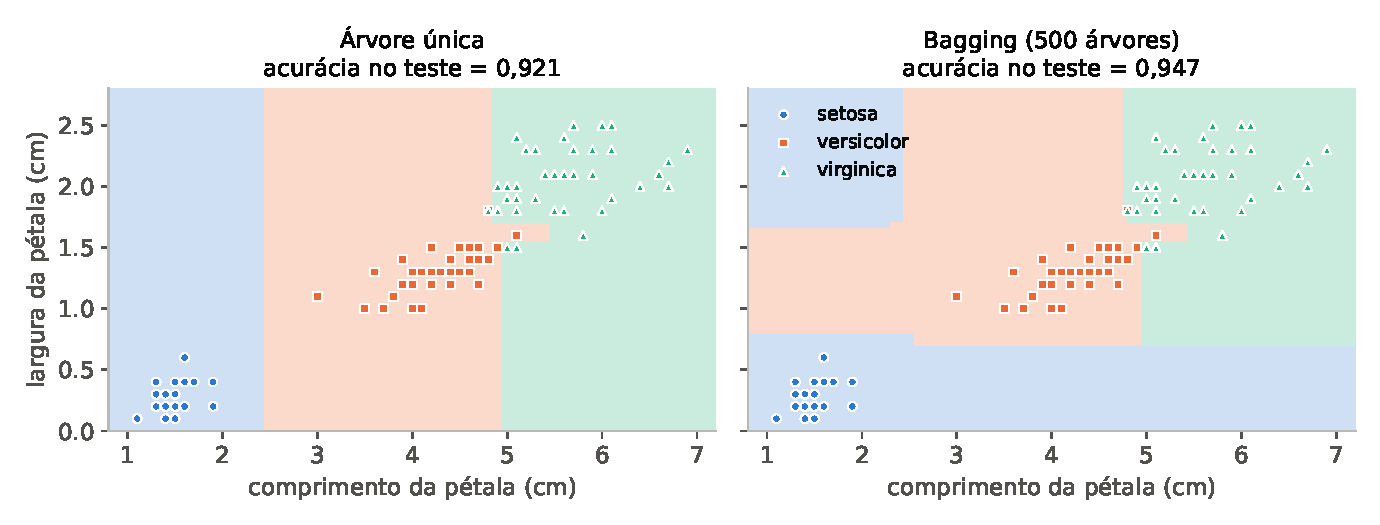
\includegraphics[width=0.84\linewidth]{../python/ensembles/figures/fronteiras_arvore_bagging.pdf}
\vspace{2pt}
\begin{itemize}
  \item Usamos só as duas variáveis da pétala para poder desenhar a fronteira. Treino: $0{,}991$ nos dois; teste: $0{,}921\to0{,}947$ (uma flor).
  \item Na região onde \emph{versicolor} e \emph{virginica} se encontram, cada árvore corta em um lugar ligeiramente diferente; o bagging vota entre esses cortes e a fronteira resultante tem \alert{mais degraus}, mas \alert{não é visivelmente mais suave} que a da árvore única.
\end{itemize}
\end{frame}

\begin{frame}{Quantas árvores? Repetindo 30 divisões}
\begin{columns}[T]
\column{0.56\textwidth}
\centering
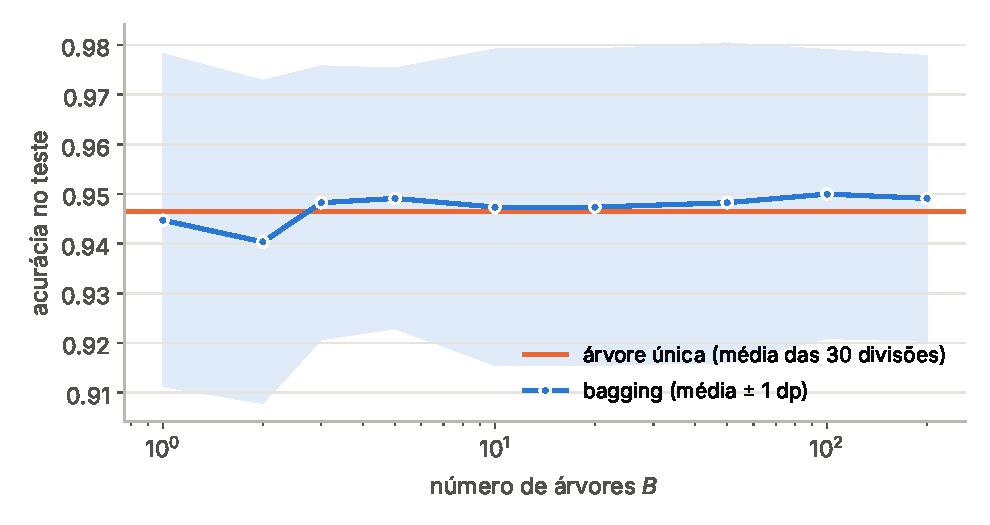
\includegraphics[width=\linewidth]{../python/ensembles/figures/acuracia_vs_B.pdf}
\column{0.42\textwidth}
\small
\begin{itemize}
  \item Árvore única: $0{,}946$ (média).
  \item Bagging: de $0{,}945$ ($B=1$) a $0{,}949$ ($B=200$).
  \item A curva é \alert{praticamente plana}: o ganho ($\approx0{,}3$ p.p.) está muito abaixo do desvio-padrão ($\approx0{,}03$).
  \item Mais árvores não pioram o resultado, mas no Iris também quase não melhoram: há pouca variância a remover.
\end{itemize}
\end{columns}
\end{frame}

\begin{frame}[fragile]{Avaliação \emph{out-of-bag} (OOB)}
Cada árvore não vê $\approx36{,}8\%$ dos pontos de treino; usam-se esses pontos como validação gratuita.

\vspace{4pt}
\lstinputlisting[style=py,firstline=10,lastline=16]{../python/ensembles/05_oob.py}
\vspace{2pt}
{\footnotesize\textbf{Saída}}
\lstinputlisting[style=saida]{../python/ensembles/outputs/05_oob.txt}
\vspace{2pt}
\begin{itemize}
  \item A estimativa OOB ($0{,}946$) fica muito próxima da acurácia de teste ($0{,}947$), sem separar dados de validação.
\end{itemize}
\end{frame}

\begin{frame}{Por que reduz a variância}
Se $\hat f_1,\dots,\hat f_B$ têm variância $\sigma^2$ e correlação par a par $\rho$:
\[
\Var\Bigl(\frac1B\sum_{b=1}^B\hat f_b\Bigr)=\rho\,\sigma^2+\frac{1-\rho}{B}\,\sigma^2 .
\]
\begin{itemize}
  \item Com $\rho=0$ (independentes): variância cai por $B$.
  \item Com $B\to\infty$: sobra $\rho\sigma^2$, o \alert{piso} imposto pela correlação entre as árvores.
  \item O viés praticamente não muda: bagging atua sobre árvores profundas (baixo viés, alta variância).
  \item Árvores de bootstrap são \alert{correlacionadas}: variáveis fortes dominam o topo de todas elas $\Rightarrow$ motivação das florestas.
\end{itemize}
\end{frame}

% =====================================================================
\section{Boosting}\label{sec:boosting}

\begin{frame}{Ideia: aprendizes fracos em sequência}
\begin{itemize}
  \item Bagging/florestas: árvores \alert{independentes} e profundas, reduzem variância.
  \item Boosting: árvores \alert{sequenciais} e rasas, cada uma corrige os erros da anterior, reduzem viés.
  \item Abordagem \alert{gulosa em modelo aditivo}:
  \[
  \hat f(\mathbf x)=\sum_{b=1}^{B}\beta_b\,T_b(\mathbf x).
  \]
  \item Duas variantes tratadas aqui: \textbf{AdaBoost} (reponderação de observações) e \textbf{gradient boosting} (ajuste a resíduos).
\end{itemize}
% [MANIM] pesos das observações mudando a cada iteração
\end{frame}

\begin{frame}[t]{Algoritmo \aAda: AdaBoost ($y_i\in\{-1,+1\}$)}
\small
\begin{algorithmic}[1]
\State $w_i\gets1/n$, \ $i=1,\dots,n$
\For{$b=1,\dots,B$}
  \State ajustar uma árvore rasa $G_b$ aos dados com pesos $w_i$
  \State $\text{err}_b\gets\dfrac{\sum_i w_i\,\ind(y_i\ne G_b(\mathbf x_i))}{\sum_i w_i}$
  \State $\alpha_b\gets\log\dfrac{1-\text{err}_b}{\text{err}_b}$
  \State $w_i\gets w_i\exp\bigl(\alpha_b\,\ind(y_i\ne G_b(\mathbf x_i))\bigr)$, \ $i=1,\dots,n$
\EndFor
\State \Return $\hat f(\mathbf x)=\operatorname{sinal}\Bigl(\sum_{b=1}^B\alpha_b\,G_b(\mathbf x)\Bigr)$
\end{algorithmic}
\vspace{6pt}
\begin{itemize}
  \item Observações erradas ganham peso; árvores mais precisas ganham $\alpha_b$ maior.
  \item Árvores usuais: poucos nós (até \emph{stumps}, com 1 divisão).
\end{itemize}
\end{frame}

\begin{frame}[t]{Algoritmo \aGB: gradient boosting para regressão (perda quadrática)}
\small
\begin{algorithmic}[1]
\State $\hat f(\mathbf x)\gets0$; \ $r_i\gets y_i$, \ $i=1,\dots,n$
\For{$b=1,\dots,B$}
  \State ajustar uma árvore $\hat f^{\,b}$ com $d$ divisões a $\{(\mathbf x_i,r_i)\}_{i=1}^n$ \Comment{\textsc{CresceÁrvore} com $h_{\max}$ pequeno}
  \State $\hat f(\mathbf x)\gets\hat f(\mathbf x)+\lambda\,\hat f^{\,b}(\mathbf x)$
  \State $r_i\gets r_i-\lambda\,\hat f^{\,b}(\mathbf x_i)$
\EndFor
\State \Return $\hat f(\mathbf x)=\sum_{b=1}^B\lambda\,\hat f^{\,b}(\mathbf x)$
\end{algorithmic}
\vspace{6pt}
\begin{itemize}
  \item Os resíduos $r_i$ são o \alert{gradiente negativo} da perda quadrática $\tfrac12(y_i-f(\mathbf x_i))^2$: é o $L_2$-boosting do livro.
  \item Parâmetros: $B$ (nº de árvores), $\lambda$ (taxa de aprendizado, p.\ ex.\ $0{,}01$--$0{,}1$), $d$ (tamanho de cada árvore).
  \item Perdas gerais (logística, etc.): ajustar a árvore ao gradiente negativo da perda.
\end{itemize}
{\footnotesize James et al.\ (2013, Alg.~8.2); Friedman (2001).}
\end{frame}

\begin{frame}{Boosting: cuidados}
\begin{itemize}
  \item Diferente de florestas, $B$ grande \alert{pode} sobreajustar: escolher $B$ por validação cruzada ou parada antecipada.
  \item Trade-off $\lambda$ \emph{versus} $B$: $\lambda$ menor exige $B$ maior, e costuma generalizar melhor.
  \item Implementações modernas (XGBoost, LightGBM, CatBoost) acrescentam regularização, \emph{subsampling} e otimizações de busca de cortes.
\end{itemize}
\end{frame}

\begin{frame}{Comparação dos métodos}
\small
\centering
\begin{tabular}{p{0.17\textwidth}p{0.14\textwidth}p{0.22\textwidth}p{0.17\textwidth}p{0.15\textwidth}}
\toprule
\textbf{Método} & \textbf{Árvores} & \textbf{Constrói} & \textbf{Reduz} & \textbf{Interpret.}\\
\midrule
Árvore única & 1 & recursivamente & --- & alta\\
Bagging & $B$, profundas & em paralelo & variância & média--baixa\\
Floresta aleatória & $B$, profundas & em paralelo, com sorteio de $m$ preditores & variância (descorrelaciona) & baixa\\
Boosting & $B$, rasas & em sequência & viés & baixa\\
\bottomrule
\end{tabular}

\vspace{8pt}
\raggedright
{\footnotesize Tendências gerais; o desempenho depende do problema e do ajuste dos hiperparâmetros.}
\end{frame}

\begin{frame}[fragile]{API do scikit-learn: \texttt{AdaBoostClassifier} e \texttt{GradientBoosting*}}
\begin{lstlisting}[style=py]
AdaBoostClassifier(estimator=None, *, n_estimators=50, learning_rate=1.0, random_state=None)
GradientBoostingRegressor(*, loss='squared_error', learning_rate=0.1, n_estimators=100,
                          subsample=1.0, max_depth=3, min_samples_leaf=1, random_state=None, ...)
\end{lstlisting}
\vspace{2pt}
\footnotesize
\begin{tabular}{@{}p{0.27\linewidth}p{0.67\linewidth}@{}}
\toprule
\texttt{n\_estimators} & número $B$ de árvores\\
\texttt{learning\_rate} & $\lambda$: encolhe a contribuição de cada árvore (no AdaBoost, multiplica $\alpha_b$)\\
\texttt{estimator} / \texttt{max\_depth} & tamanho das árvores: \emph{stumps} (\texttt{max\_depth=1}) no AdaBoost; $d$ pequeno no gradient boosting\\
\texttt{subsample} & fração das observações sorteada a cada árvore ($<1$: \emph{stochastic} GB)\\
\bottomrule
\end{tabular}

\vspace{2pt}
{\scriptsize Versão 1.9. Classificação com gradient boosting: \texttt{GradientBoostingClassifier}, mesmos parâmetros.}
\end{frame}

\begin{frame}[fragile]{Exemplo em Python: AdaBoost com \emph{stumps}}
\lstinputlisting[style=py,basicstyle=\ttfamily\fontsize{7}{8.4}\selectfont]{../python/boosting/01_adaboost.py}
\lstinputlisting[style=saida,basicstyle=\ttfamily\fontsize{7}{8.4}\selectfont]{../python/boosting/outputs/01_adaboost.txt}
\vspace{2pt}
{\small Um \emph{stump} sozinho ($B=1$) só separa uma espécie das outras ($0{,}658$); $10$ deles chegam a $0{,}921$. Depois disso a curva oscila ($0{,}895$ em $B=50$): com $38$ flores de teste, $0{,}026$ é \alert{uma} flor.}
\end{frame}

\begin{frame}[fragile]{Exemplo em Python: gradient boosting do zero (Alg.~\aGB)}
\lstinputlisting[style=py,basicstyle=\ttfamily\fontsize{7}{8.4}\selectfont,firstline=10,lastline=25]{../python/boosting/02_gb_do_zero.py}
\vspace{3pt}
\lstinputlisting[style=saida,basicstyle=\ttfamily\fontsize{7}{8.4}\selectfont]{../python/boosting/outputs/02_gb_do_zero.txt}
\vspace{2pt}
{\small Dados \emph{diabetes} (todas as $10$ variáveis). Cada árvore ajusta os \alert{resíduos}; a soma com $\lambda=0{,}1$ reproduz o \texttt{GradientBoostingRegressor} (mesmo RMSE). Diferença para o Alg.~\aGB: aqui $\hat f_0=\bar y$ em vez de $0$ (o scikit-learn faz o mesmo).}
\end{frame}

\begin{frame}{Árvore, bagging e boosting: métricas no Iris}
\centering
\small
\begin{tabular}{@{}lcc@{}}
\toprule
Método & Acurácia & F1 macro \\
\midrule
Árvore (Gini) & 0,946 $\pm$ 0,033 & 0,946 $\pm$ 0,033 \\
Árvore (entropia) & 0,944 $\pm$ 0,032 & 0,944 $\pm$ 0,032 \\
Bagging ($B=200$) & 0,952 $\pm$ 0,030 & 0,952 $\pm$ 0,030 \\
AdaBoost ($B=200$, \emph{stumps}) & 0,941 $\pm$ 0,032 & 0,941 $\pm$ 0,032 \\
Gradient boosting ($B=100$, $d=2$) & 0,948 $\pm$ 0,030 & 0,948 $\pm$ 0,029 \\
\bottomrule
\end{tabular}


\vspace{4pt}
\raggedright
{\footnotesize Média $\pm$ desvio-padrão em $100$ divisões estratificadas $75/25$ (mesmas divisões para todos os métodos); hiperparâmetros fixados antes, sem ajuste. Código: \texttt{03\_tabela\_comparacao.py}.}
\begin{itemize}
  \item \alert{Gini $\times$ entropia}: $0{,}946$ \emph{versus} $0{,}944$, diferença de $0{,}002$ para um desvio-padrão de $0{,}03$. Na prática, escolha irrelevante aqui.
  \item Bagging e gradient boosting ficam $\approx0{,}2$--$0{,}6$ p.p.\ acima da árvore; AdaBoost, $0{,}5$ abaixo. Tudo \alert{dentro de um desvio-padrão}: o Iris é fácil demais para separar os métodos.
  \item A acurácia e o F1 macro coincidem porque as três classes são balanceadas.
\end{itemize}
\end{frame}

% =====================================================================

\section{Caso prático}\label{sec:caso}

\begin{frame}{Comparativos}
Duas tarefas, dois conjuntos \alert{disponíveis no scikit-learn} (sem download):
\begin{itemize}
  \item \textbf{Classificação}: Iris ($150$ flores, $4$ medidas, $3$ espécies).
  \item \textbf{Regressão}: \emph{diabetes} ($442$ pacientes, $10$ variáveis, resposta: progressão da doença).
\end{itemize}
Pergunta: \alert{quando vale a pena usar árvores}, comparadas com \alert{baselines} (regressão linear/logística, KNN, LDA, SVM)?
\begin{enumerate}
  \item Protocolo de avaliação.
  \item Classificação: árvores $\times$ baselines.
  \item Regressão: árvores (e ensembles) $\times$ baselines.
  \item Duas propriedades das árvores: \alert{escala} e \alert{rotação} dos eixos.
  \item Resumo: o que levar para a prática.
\end{enumerate}
\end{frame}

\begin{frame}{Protocolo de avaliação}
\begin{itemize}
  \item \alert{Repetir} a divisão treino/teste ($75/25$): $100$ vezes no Iris (estratificado), $50$ no \emph{diabetes}. Com $38$ flores de teste, uma observação vale $2{,}6$ p.p.; uma única divisão não decide.
  \item Relatamos \alert{média $\pm$ desvio-padrão} entre as divisões. Diferenças menores que o desvio-padrão \alert{não} devem ser lidas como superioridade.
  \item Pré-processamento \alert{dentro} do \texttt{Pipeline}: a padronização (para KNN, SVM e regressão logística) é ajustada só com o treino de cada divisão, evitando \emph{vazamento}.
  \item Hiperparâmetros \alert{fixados antes}, sem ajuste fino para nenhum método (ver código). Um ajuste por validação cruzada pode mudar a ordem entre métodos próximos.
\end{itemize}
\end{frame}

\begin{frame}[fragile]{Classificação (Iris): árvores $\times$ baselines}
\centering\small
\begin{tabular}{@{}lcc@{}}
\toprule
Método & Acurácia & F1 macro \\
\midrule
Regressão logística & 0,954 $\pm$ 0,028 & 0,954 $\pm$ 0,028 \\
KNN ($k=5$) & 0,950 $\pm$ 0,031 & 0,950 $\pm$ 0,030 \\
LDA & 0,982 $\pm$ 0,018 & 0,982 $\pm$ 0,018 \\
SVM (RBF) & 0,960 $\pm$ 0,028 & 0,960 $\pm$ 0,028 \\
Árvore (prof.\ 3) & 0,943 $\pm$ 0,032 & 0,943 $\pm$ 0,032 \\
Árvore (completa) & 0,946 $\pm$ 0,033 & 0,946 $\pm$ 0,033 \\
\bottomrule
\end{tabular}


\vspace{4pt}
\raggedright
\begin{itemize}
  \item \alert{LDA lidera} ($0{,}982$): as classes são quase \alert{linearmente separáveis} e aproximadamente gaussianas com covariâncias parecidas, o que o LDA supõe.
  \item SVM, regressão logística e KNN: $0{,}950$--$0{,}960$. As árvores: $0{,}943$--$0{,}946$, \alert{abaixo} dos baselines, mas por menos de $2$ desvios-padrão ($\approx0{,}03$).
  \item A árvore de profundidade $3$ empata com a completa e cabe em um slide: aqui a árvore compra \alert{interpretabilidade} quase sem custo.
\end{itemize}
{\scriptsize Código: \texttt{01\_baselines\_classificacao.py}.}
\end{frame}

\begin{frame}{Regressão (\emph{diabetes}): árvores $\times$ baselines}
\centering\small
\begin{tabular}{@{}lcc@{}}
\toprule
Método & RMSE & $R^2$ \\
\midrule
Regressão linear & 54,9 $\pm$ 2,7 & 0,47 $\pm$ 0,05 \\
KNN ($k=15$) & 57,0 $\pm$ 3,2 & 0,43 $\pm$ 0,05 \\
SVR (RBF, $C=100$) & 57,9 $\pm$ 3,9 & 0,41 $\pm$ 0,08 \\
Árvore (prof.\ 3) & 63,0 $\pm$ 3,7 & 0,30 $\pm$ 0,10 \\
Árvore (completa) & 80,1 $\pm$ 4,8 & -0,12 $\pm$ 0,15 \\
Floresta ($B=300$) & 57,3 $\pm$ 3,6 & 0,43 $\pm$ 0,08 \\
Gradient boosting & 56,7 $\pm$ 3,1 & 0,44 $\pm$ 0,06 \\
\bottomrule
\end{tabular}


\vspace{4pt}
\raggedright
\begin{itemize}
  \item A \alert{regressão linear} vence ($54{,}9$): a relação resposta--variáveis é aproximadamente linear.
  \item \alert{Árvore completa}: RMSE $80{,}1$ e $R^2<0$, \alert{pior que prever a média}. Poda (prof.\ $3$) melhora para $63{,}0$.
  \item Floresta e gradient boosting ($56{,}7$--$57{,}3$) recuperam quase todo o terreno perdido pela árvore, e ficam a $\approx2$ pontos da regressão linear, dentro de $1$ desvio-padrão.
\end{itemize}
{\scriptsize Código: \texttt{02\_baselines\_regressao.py}. Hiperparâmetros fixados antes, sem ajuste.}
\end{frame}

\begin{frame}{Propriedade 1: indiferença à escala das variáveis}
\begin{columns}[T]
\column{0.5\textwidth}
\centering\footnotesize
\begin{tabular}{@{}lcc@{}}
\toprule
Método & Original & Variável 1 $\times\,1000$ \\
\midrule
KNN & 0,964 & 0,759 \\
SVM (RBF) & 0,959 & 0,684 \\
Regressão logística & 0,963 & 0,959 \\
LDA & 0,981 & 0,981 \\
Árvore (prof.\ 3) & 0,939 & 0,939 \\
\bottomrule
\end{tabular}


\vspace{4pt}
{\scriptsize Acurácia média no Iris ($50$ divisões), \alert{sem} padronizar; a variável $1$ (comprimento da sépala) é multiplicada por $1000$.}
\column{0.47\textwidth}
\small
\begin{itemize}
  \item \alert{KNN} e \alert{SVM} dependem de \alert{distâncias}: a variável $\times1000$ domina e a acurácia cai $20$--$28$ p.p.
  \item A \alert{árvore} só usa a \alert{ordem} dos valores em cada variável: a partição dos dados de treino \alert{não muda}.
  \item LDA é invariante a escalas lineares. A regressão logística mal muda ($0{,}963\to0{,}959$): a regularização $L_2$ depende da escala.
\end{itemize}
\end{columns}
\vspace{4pt}
\begin{block}{Consequência}
Árvores dispensam padronização, e qualquer transformação \alert{estritamente crescente} de uma variável (log, raiz) deixa a partição do treino igual.
\end{block}
\end{frame}

\begin{frame}{Propriedade 2: a rotação dos eixos}
\centering
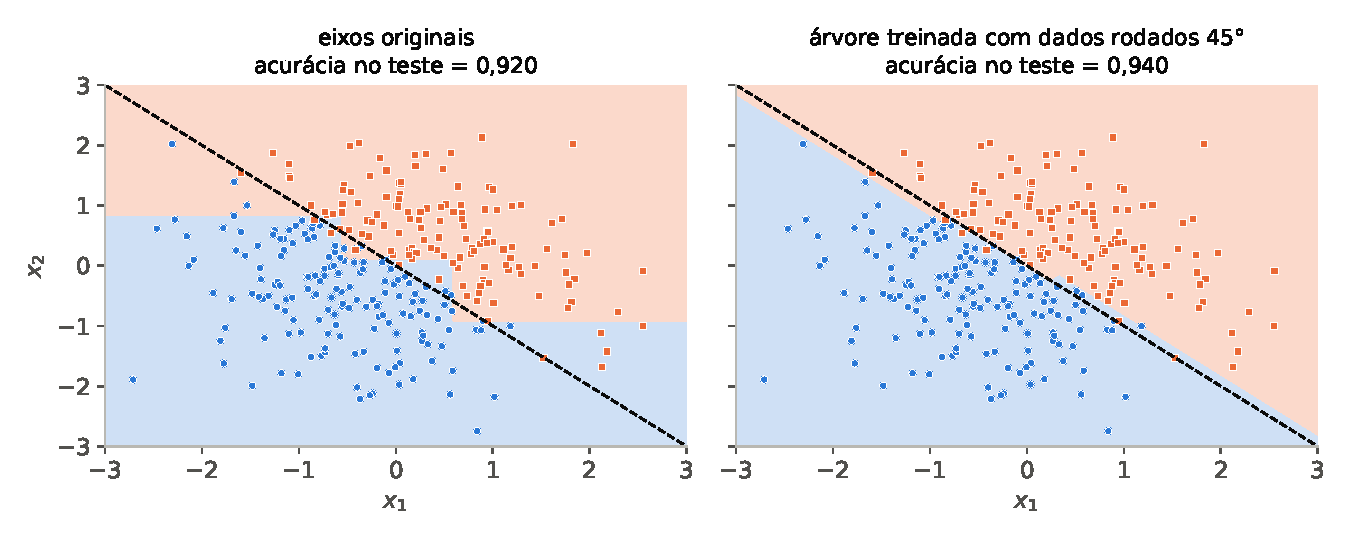
\includegraphics[width=0.62\linewidth]{../python/comparativo/figures/rotacao.pdf}
\vspace{2pt}
\begin{itemize}
  \item Cortes $x_j\le\tau$ dão fronteiras \alert{paralelas aos eixos}: uma fronteira \alert{diagonal} ($x_1+x_2=0$) vira uma \alert{escada}.
  \item Sintéticos ($50$ divisões, prof.\ $3$): árvore $0{,}891$; com dados \alert{rodados $45^\circ$} $0{,}968$; regressão logística $0{,}976$.
  \item Mas depende da \alert{geometria}: no Iris, rodar os $4$ eixos por uma matriz ortogonal aleatória \alert{não} prejudicou ($0{,}939\to0{,}937$).
\end{itemize}
{\scriptsize Código: \texttt{04\_rotacao.py}, \texttt{fig\_rotacao.py}.}
\end{frame}

\begin{frame}{Resumo: o que levar para a prática}
\small
\centering
\begin{tabular}{@{}p{0.2\textwidth}p{0.24\textwidth}p{0.24\textwidth}p{0.2\textwidth}@{}}
\toprule
 & \textbf{Árvore} & \textbf{Linear / LDA} & \textbf{KNN / SVM}\\
\midrule
Escala das variáveis & indiferente & LDA: indiferente & \alert{sensível}\\
Rotação dos eixos & \alert{sensível} (fronteira diagonal) & indiferente & indiferente\\
Interpretação & alta (regras) & alta (coeficientes) & baixa\\
Extrapolação & constante (degraus) & linear & tende a constante\\
\bottomrule
\end{tabular}

\vspace{6pt}
\raggedright
\begin{itemize}
  \item Nos dois conjuntos, \alert{uma árvore sozinha não vence} os baselines; floresta e boosting chegam perto.
  \item Árvores costumam brilhar com variáveis em unidades distintas, interações e mistura de tipos (que o Iris e o \emph{diabetes} não testam); sempre \alert{compare com um baseline simples}.
\end{itemize}
\end{frame}


% =====================================================================
\section{Conclusões}

\begin{frame}{Conclusões}
\begin{itemize}
  \item Árvore = partição do espaço em retângulos $p$-dimensionais com previsão constante em cada região.
  \item CART: a cada nó, uma pergunta sobre uma variável que minimiza o erro, repetida recursivamente; precisa de condição de parada e termina com no máximo $n$ folhas.
  \item Gini e entropia (côncavas) garantem $\Delta\ge0$ e funcionam melhor que o erro para \alert{crescer}; o erro serve à \alert{poda}.
  \item Profundidade controla viés--variância: pré-poda, pós-poda por custo-complexidade e validação cruzada.
  \item Bagging e florestas (spoiler de florestas aleatorias) reduzem variância; boosting reduz viés; todos pagam em interpretabilidade.
  \item Na prática (Iris e \emph{diabetes}): uma árvore sozinha não venceu os baselines; floresta e boosting chegam perto. Árvores são \alert{indiferentes à escala}, mas \alert{sensíveis à rotação} dos eixos quando a fronteira é diagonal.
\end{itemize}
\end{frame}

\begin{frame}[allowframebreaks]{Referências}
\footnotesize
\begin{thebibliography}{99}
\bibitem{ms} Morettin, P.\ A.; Singer, J.\ M. \textit{Estatística e Ciência de Dados}. Versão preliminar, abril de 2021. Departamento de Estatística, USP. Cap.~10.
\bibitem{geron} Géron, A. \textit{Hands-On Machine Learning with Scikit-Learn, Keras, and TensorFlow}. 3rd ed., O'Reilly, 2022. Caps.~6 e 7.
\bibitem{esl} Hastie, T.; Tibshirani, R.; Friedman, J. \textit{The Elements of Statistical Learning}. 2nd ed., Springer, 2009. Caps.~9, 10 e 15.
\bibitem{isl} James, G.; Witten, D.; Hastie, T.; Tibshirani, R. \textit{An Introduction to Statistical Learning}. Springer, 2013. Cap.~8.
\bibitem{hr} Hyafil, L.; Rivest, R.\ L. Constructing optimal binary decision trees is NP-complete. \textit{Information Processing Letters}, 5(1), 1976.
\bibitem{ada} Freund, Y.; Schapire, R.\ E. A decision-theoretic generalization of on-line learning and an application to boosting. \textit{Journal of Computer and System Sciences}, 55, 1997.
\bibitem{gb} Friedman, J.\ H. Greedy function approximation: a gradient boosting machine. \textit{The Annals of Statistics}, 29(5), 2001.
\end{thebibliography}
\end{frame}

\end{document}